% Options for packages loaded elsewhere
\PassOptionsToPackage{unicode}{hyperref}
\PassOptionsToPackage{hyphens}{url}
%
\documentclass[
]{book}
\usepackage{amsmath,amssymb}
\usepackage{iftex}
\ifPDFTeX
  \usepackage[T1]{fontenc}
  \usepackage[utf8]{inputenc}
  \usepackage{textcomp} % provide euro and other symbols
\else % if luatex or xetex
  \usepackage{unicode-math} % this also loads fontspec
  \defaultfontfeatures{Scale=MatchLowercase}
  \defaultfontfeatures[\rmfamily]{Ligatures=TeX,Scale=1}
\fi
\usepackage{lmodern}
\ifPDFTeX\else
  % xetex/luatex font selection
\fi
% Use upquote if available, for straight quotes in verbatim environments
\IfFileExists{upquote.sty}{\usepackage{upquote}}{}
\IfFileExists{microtype.sty}{% use microtype if available
  \usepackage[]{microtype}
  \UseMicrotypeSet[protrusion]{basicmath} % disable protrusion for tt fonts
}{}
\makeatletter
\@ifundefined{KOMAClassName}{% if non-KOMA class
  \IfFileExists{parskip.sty}{%
    \usepackage{parskip}
  }{% else
    \setlength{\parindent}{0pt}
    \setlength{\parskip}{6pt plus 2pt minus 1pt}}
}{% if KOMA class
  \KOMAoptions{parskip=half}}
\makeatother
\usepackage{xcolor}
\usepackage{color}
\usepackage{fancyvrb}
\newcommand{\VerbBar}{|}
\newcommand{\VERB}{\Verb[commandchars=\\\{\}]}
\DefineVerbatimEnvironment{Highlighting}{Verbatim}{commandchars=\\\{\}}
% Add ',fontsize=\small' for more characters per line
\usepackage{framed}
\definecolor{shadecolor}{RGB}{248,248,248}
\newenvironment{Shaded}{\begin{snugshade}}{\end{snugshade}}
\newcommand{\AlertTok}[1]{\textcolor[rgb]{0.94,0.16,0.16}{#1}}
\newcommand{\AnnotationTok}[1]{\textcolor[rgb]{0.56,0.35,0.01}{\textbf{\textit{#1}}}}
\newcommand{\AttributeTok}[1]{\textcolor[rgb]{0.13,0.29,0.53}{#1}}
\newcommand{\BaseNTok}[1]{\textcolor[rgb]{0.00,0.00,0.81}{#1}}
\newcommand{\BuiltInTok}[1]{#1}
\newcommand{\CharTok}[1]{\textcolor[rgb]{0.31,0.60,0.02}{#1}}
\newcommand{\CommentTok}[1]{\textcolor[rgb]{0.56,0.35,0.01}{\textit{#1}}}
\newcommand{\CommentVarTok}[1]{\textcolor[rgb]{0.56,0.35,0.01}{\textbf{\textit{#1}}}}
\newcommand{\ConstantTok}[1]{\textcolor[rgb]{0.56,0.35,0.01}{#1}}
\newcommand{\ControlFlowTok}[1]{\textcolor[rgb]{0.13,0.29,0.53}{\textbf{#1}}}
\newcommand{\DataTypeTok}[1]{\textcolor[rgb]{0.13,0.29,0.53}{#1}}
\newcommand{\DecValTok}[1]{\textcolor[rgb]{0.00,0.00,0.81}{#1}}
\newcommand{\DocumentationTok}[1]{\textcolor[rgb]{0.56,0.35,0.01}{\textbf{\textit{#1}}}}
\newcommand{\ErrorTok}[1]{\textcolor[rgb]{0.64,0.00,0.00}{\textbf{#1}}}
\newcommand{\ExtensionTok}[1]{#1}
\newcommand{\FloatTok}[1]{\textcolor[rgb]{0.00,0.00,0.81}{#1}}
\newcommand{\FunctionTok}[1]{\textcolor[rgb]{0.13,0.29,0.53}{\textbf{#1}}}
\newcommand{\ImportTok}[1]{#1}
\newcommand{\InformationTok}[1]{\textcolor[rgb]{0.56,0.35,0.01}{\textbf{\textit{#1}}}}
\newcommand{\KeywordTok}[1]{\textcolor[rgb]{0.13,0.29,0.53}{\textbf{#1}}}
\newcommand{\NormalTok}[1]{#1}
\newcommand{\OperatorTok}[1]{\textcolor[rgb]{0.81,0.36,0.00}{\textbf{#1}}}
\newcommand{\OtherTok}[1]{\textcolor[rgb]{0.56,0.35,0.01}{#1}}
\newcommand{\PreprocessorTok}[1]{\textcolor[rgb]{0.56,0.35,0.01}{\textit{#1}}}
\newcommand{\RegionMarkerTok}[1]{#1}
\newcommand{\SpecialCharTok}[1]{\textcolor[rgb]{0.81,0.36,0.00}{\textbf{#1}}}
\newcommand{\SpecialStringTok}[1]{\textcolor[rgb]{0.31,0.60,0.02}{#1}}
\newcommand{\StringTok}[1]{\textcolor[rgb]{0.31,0.60,0.02}{#1}}
\newcommand{\VariableTok}[1]{\textcolor[rgb]{0.00,0.00,0.00}{#1}}
\newcommand{\VerbatimStringTok}[1]{\textcolor[rgb]{0.31,0.60,0.02}{#1}}
\newcommand{\WarningTok}[1]{\textcolor[rgb]{0.56,0.35,0.01}{\textbf{\textit{#1}}}}
\usepackage{longtable,booktabs,array}
\usepackage{calc} % for calculating minipage widths
% Correct order of tables after \paragraph or \subparagraph
\usepackage{etoolbox}
\makeatletter
\patchcmd\longtable{\par}{\if@noskipsec\mbox{}\fi\par}{}{}
\makeatother
% Allow footnotes in longtable head/foot
\IfFileExists{footnotehyper.sty}{\usepackage{footnotehyper}}{\usepackage{footnote}}
\makesavenoteenv{longtable}
\usepackage{graphicx}
\makeatletter
\def\maxwidth{\ifdim\Gin@nat@width>\linewidth\linewidth\else\Gin@nat@width\fi}
\def\maxheight{\ifdim\Gin@nat@height>\textheight\textheight\else\Gin@nat@height\fi}
\makeatother
% Scale images if necessary, so that they will not overflow the page
% margins by default, and it is still possible to overwrite the defaults
% using explicit options in \includegraphics[width, height, ...]{}
\setkeys{Gin}{width=\maxwidth,height=\maxheight,keepaspectratio}
% Set default figure placement to htbp
\makeatletter
\def\fps@figure{htbp}
\makeatother
\ifLuaTeX
  \usepackage{luacolor}
  \usepackage[soul]{lua-ul}
\else
  \usepackage{soul}
\fi
\setlength{\emergencystretch}{3em} % prevent overfull lines
\providecommand{\tightlist}{%
  \setlength{\itemsep}{0pt}\setlength{\parskip}{0pt}}
\setcounter{secnumdepth}{5}
\usepackage{booktabs}
\usepackage{amssymb}
\usepackage{amsmath}
\usepackage{graphicx}
\usepackage{wasysym}
\usepackage{amsthm}
\usepackage{multirow}
\usepackage{epsf}
\usepackage{tikz}
\usepackage{cancel}
\usepackage{hyperref}
\usepackage{gensymb}
\usepackage{color}
\usepackage{framed}
\setlength{\fboxsep}{.8em}

\newenvironment{blackbox}{
  \definecolor{shadecolor}{rgb}{0, 0, 0}  % black
  \color{white}
  \begin{shaded}}
 {\end{shaded}}
\ifLuaTeX
  \usepackage{selnolig}  % disable illegal ligatures
\fi
\usepackage[]{natbib}
\bibliographystyle{plainnat}
\usepackage{bookmark}
\IfFileExists{xurl.sty}{\usepackage{xurl}}{} % add URL line breaks if available
\urlstyle{same}
\hypersetup{
  pdftitle={Bookdown: Flexible Document Creation in RStudio},
  pdfauthor={Joseph Thiers},
  hidelinks,
  pdfcreator={LaTeX via pandoc}}

\title{Bookdown: Flexible Document Creation in RStudio}
\usepackage{etoolbox}
\makeatletter
\providecommand{\subtitle}[1]{% add subtitle to \maketitle
  \apptocmd{\@title}{\par {\large #1 \par}}{}{}
}
\makeatother
\subtitle{Guide for Students, Researchers, and Professionals}
\author{Joseph Thiers}
\date{}

\usepackage{amsthm}
\newtheorem{theorem}{Theorem}[chapter]
\newtheorem{lemma}{Lemma}[chapter]
\newtheorem{corollary}{Corollary}[chapter]
\newtheorem{proposition}{Proposition}[chapter]
\newtheorem{conjecture}{Conjecture}[chapter]
\theoremstyle{definition}
\newtheorem{definition}{Definition}[chapter]
\theoremstyle{definition}
\newtheorem{example}{Example}[chapter]
\theoremstyle{definition}
\newtheorem{exercise}{Exercise}[chapter]
\theoremstyle{definition}
\newtheorem{hypothesis}{Hypothesis}[chapter]
\theoremstyle{remark}
\newtheorem*{remark}{Remark}
\newtheorem*{solution}{Solution}
\begin{document}
\maketitle

{
\setcounter{tocdepth}{1}
\tableofcontents
}
\chapter{Introduction to Bookdown}\label{introduction}

In today's fast-paced academic and professional environments, the ability to create dynamic, reproducible documents is crucial. Bookdown empowers users to combine text, code, and visualizations in a single, streamlined workflow. It is ideal for creating the type of documentation that best fits your needs, whether that be single-page assignments, reports, academic papers, or even full-length books.

\section{Why RStudio and Bookdown?}\label{why-rstudio-and-bookdown}

Bookdown offers a range of benefits:
- Seamlessly integrates text, code, and figures.
- Supports multiple output formats (HTML, PDF, EPUB).
- Simplifies the creation of reproducible and professional documents.
- Ideal for mathematics, statistics, and data science professionals.

\section{What You'll Learn in This Tutorial}\label{what-youll-learn-in-this-tutorial}

This tutorial will guide you through the essential aspects of using Bookdown:

\begin{itemize}
\tightlist
\item
  \textbf{Chapter \ref{introduction}}: Introduction to Bookdown -- Learn about its purpose and benefits for structured documentation.
\item
  \textbf{Chapter \ref{chapter2}}: Getting Started -- Install R, RStudio, and Bookdown, create a project, and render your first book.
\item
  \textbf{Chapter \ref{chapter3}}: Writing Content -- Organize chapters, use Markdown, format text, add code chunks, and images.
\item
  \textbf{Chapter \ref{chapter4}}: Cross-Referencing -- Reference sections, figures, tables, and equations effectively.
\item
  \textbf{Chapter \ref{chapter5}}: LaTeX -- Add equations, theorems, lemmas, and proofs.
\item
  \textbf{Chapter \ref{chapter6}}: Advanced Features -- Manage citations, use LaTeX packages, and more!
\item
  \textbf{Chapter \ref{chapter7}}: Customizing Output -- Configure formats like HTML, PDF, and EPUB, and style your book with CSS or LaTeX.
\item
  \textbf{Chapter \ref{latexdistributions}}: LaTeX Distributions - Different distributions available.
\item
  \textbf{Chapter \ref{markdownadvanced}}: Advanced Text Formatting Options - Advanced Markdown and Pandoc code to stylize the book to your needs.
\item
  \textbf{Chapter \ref{examplepaper}}: Example Document: Union Earnings Analysis
\end{itemize}

By the end of this tutorial, you'll have the knowledge to create, customize, and publish professional-grade documents.

\chapter{Getting Started}\label{chapter2}

To get started with Bookdown you need to install R, RStudio, Bookdown, and the LaTeX distrobution of your choice if you wish to outpute as a PDF. This can be accomplished by following these steps::

\begin{enumerate}
\def\labelenumi{\arabic{enumi}.}
\tightlist
\item
  \textbf{Install R}
  Go to the \href{https://cran.r-project.org/}{R Project download page} and download the latest version of R for your operating system (Windows, macOS, or Linux). Follow the installation instructions provided.
\end{enumerate}


\includegraphics[width=27.33in]{images/tutorialscreenshots/installR}

\begin{enumerate}
\def\labelenumi{\arabic{enumi}.}
\setcounter{enumi}{1}
\item
  \textbf{Install RStudio}:\\
  Go to the \href{https://posit.co/download/rstudio-desktop/}{RStudio download page} and select the appropriate version for your operating system. Download and follow the installation instructions.

  
\includegraphics[width=16.83in]{images/tutorialscreenshots/installRStudio}
\item
  \textbf{Install Bookdown}:\\
  Once RStudio is installed, install the Bookdown package by typing the following command in the RStudio console:

\begin{Shaded}
\begin{Highlighting}[]
\FunctionTok{install.packages}\NormalTok{(}\StringTok{"bookdown"}\NormalTok{)}
\end{Highlighting}
\end{Shaded}

  Alternatively, you can install the Bookdown package via the RStudio \textbf{Packages} pane:

  \begin{itemize}
  \item
    Select \textbf{Packages} in the bottom right-hand corner of RStudio.

    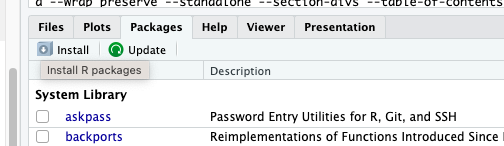
\includegraphics[width=7in]{images/tutorialscreenshots/installPackage}
  \item
    Click \textbf{Install}, type \texttt{bookdown} in the \textbf{Packages} box, and click \textbf{Install}.

    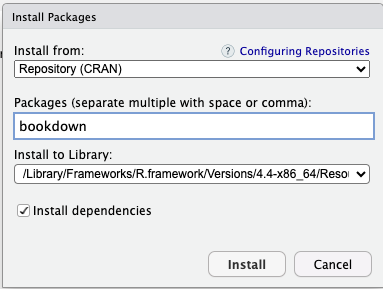
\includegraphics[width=5.32in]{images/tutorialscreenshots/installBookdownPack}
  \end{itemize}
\item
  \textbf{Install LaTeX distribution of your choice}:
  The distribution you choose is entirely up to you and your needs. For a list of recommended LaTeX distributions please see \hyperref[latexdistributions]{LaTeX Distributions Chapter \ref{latexdistributions}}
\end{enumerate}

To get started quickly TinyTeX is recommended as it can be installed from within RStudio by running the following code:

\begin{verbatim}
install.packages("tinytex")
tinytex::install_tinytex()
\end{verbatim}

Once this is complete Bookdown is now installed and you are ready to create your first Bookdown project.

\begin{enumerate}
\def\labelenumi{\arabic{enumi}.}
\setcounter{enumi}{4}
\tightlist
\item
  \textbf{Create a New Bookdown Project in RStudio}:

  \begin{itemize}
  \tightlist
  \item
    In RStudio, go to \textbf{File \textgreater{} New Project}.
  \item
    Select \textbf{New Directory} and then \textbf{Book Project using Bookdown}.
  \item
    Name your project and choose a location to save it to.
  \end{itemize}
\end{enumerate}

Now you have a newly created Bookdown project ready to be edited to fit your needs. Bookdown comes with a base set of files so that users can get started quickly with minimal fuss. Spend a few moments to explore the files in the bottom right corner of RStudio, these are the default files Bookdown creates to get you started. It even includes sample chapters for you!

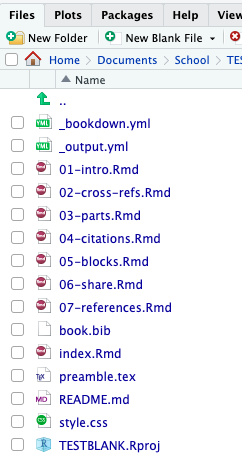
\includegraphics[width=3.36in]{images/tutorialscreenshots/filestructure}

At the end of each section is a quick exercise for you to practice on your own files.

Then when you're ready to complete your project just follow the last step below to render your book.

\begin{enumerate}
\def\labelenumi{\arabic{enumi}.}
\setcounter{enumi}{5}
\tightlist
\item
  \textbf{Render Your Newly Created Book}:\\
  In the \textbf{Build} pane:

  \begin{itemize}
  \tightlist
  \item
    Select \textbf{Build Book} and choose your output format, or select \emph{All formats} to render your files as HTML, PDF, and EPUB.
  \item
    You can also render the book directly from the R console with the following command:
  \end{itemize}

\begin{Shaded}
\begin{Highlighting}[]
\NormalTok{bookdown}\SpecialCharTok{::}\FunctionTok{render\_book}\NormalTok{(}\StringTok{"index.Rmd"}\NormalTok{)}
\end{Highlighting}
\end{Shaded}
\end{enumerate}

\chapter{Writing Content}\label{chapter3}

In this chapter, we will explore how to write and structure content in Bookdown using R Markdown syntax. Bookdown allows you to create well-organized documents by combining text, code, and references. Here, we'll cover how to organize chapters, use Markdown and LaTeX for formatting, and format text, code chunks, and images.

\begin{center}\rule{0.5\linewidth}{0.5pt}\end{center}

\section{Creating Chapters and Sections}\label{creating-chapters-and-sections}

Each chapter in Bookdown is represented by a separate \texttt{.Rmd} file, and each \texttt{.Rmd} file should begin with a first-level heading, marked by a single \texttt{\#} symbol. For example, this chapter file is \texttt{02-writing-content.Rmd} and the file starts with:

\begin{Shaded}
\begin{Highlighting}[]
\FunctionTok{\# Writing Content}
\end{Highlighting}
\end{Shaded}

\subsection{Organizing Chapters}\label{organizing-chapters}

Chapters are automatically numbered based on their order in the project directory. Ensure that each file name reflects its chapter number (e.g., \texttt{02-writing-content.Rmd} for Chapter 2).

\subsection{Adding Sections and Subsections}\label{adding-sections-and-subsections}

You can add sections and subsections within a chapter using second-level and higher-level headings:

\begin{Shaded}
\begin{Highlighting}[]
\FunctionTok{\#\# Section Title}
\FunctionTok{\#\#\# Subsection Title}
\end{Highlighting}
\end{Shaded}

This hierarchy organizes the document according to your needs, and these sections will automatically appear in the table of contents.

\begin{center}\rule{0.5\linewidth}{0.5pt}\end{center}

\section{Formatting Text in Bookdown}\label{formatting-text-in-bookdown}

Bookdown supports a wide range of Markdown formatting. Here are a few basics:

\begin{itemize}
\tightlist
\item
  \textbf{Bold}: \texttt{**bold\ text**} → \textbf{bold text}
\item
  \emph{Italics}: \texttt{*italicized\ text*} → \emph{italicized text}
\item
  \textbf{Bullet Points}:

  \begin{itemize}
  \tightlist
  \item
    First item
  \item
    Second item
  \end{itemize}
\item
  \textbf{Numbered Lists}:

  \begin{enumerate}
  \def\labelenumi{\arabic{enumi}.}
  \tightlist
  \item
    First item

    \begin{itemize}
    \tightlist
    \item
      Even sublists
    \item
      Like this
    \end{itemize}
  \item
    Second item
  \end{enumerate}
\end{itemize}

For additional text formatting options refer to \hyperref[markdown-advanced]{Chapter 9 Advanced Text Formatting}.

Use these formatting options to style text and create lists within your chapters.

\begin{center}\rule{0.5\linewidth}{0.5pt}\end{center}

\section{Adding Code Chunks}\label{adding-code-chunks}

One of the strengths of Bookdown is the ability to incorporate code into your document, whether it's R code, Markdown, LaTeX, Python, or other languages. Below are examples of how to include different types of code in your Bookdown project.

\subsection{1. R Code}\label{r-code}

R code chunks are written between three backticks (``\texttt{)\ with}\{r\}` specifying R as the language:

\begin{Shaded}
\begin{Highlighting}[]
\SpecialCharTok{\textbackslash{}\textasciigrave{}}\NormalTok{\textasciigrave{}\textasciigrave{}\{r eval=FALSE\}}
\NormalTok{summary(cars)}
\SpecialCharTok{\textbackslash{}\textasciigrave{}}\NormalTok{\textasciigrave{}\textasciigrave{}}
\end{Highlighting}
\end{Shaded}

This code will display the \texttt{summary} function output of the \texttt{cars} dataset when \texttt{eval} is set to \texttt{TRUE}.

Say you are doing data-anaylsis on the Stars dataset in the \texttt{dslabs} package.

\begin{Shaded}
\begin{Highlighting}[]
\FunctionTok{library}\NormalTok{(dslabs)}
\FunctionTok{summary}\NormalTok{(stars)}
\end{Highlighting}
\end{Shaded}

\begin{verbatim}
##           star      magnitude           temp           type          
##  Altair     : 2   Min.   :-8.000   Min.   : 2500   Length:96         
##  *40EridaniA: 1   1st Qu.:-1.800   1st Qu.: 3168   Class :character  
##  *40EridaniB: 1   Median : 2.400   Median : 5050   Mode  :character  
##  *40EridaniC: 1   Mean   : 4.257   Mean   : 8752                     
##  *61CygniA  : 1   3rd Qu.:11.325   3rd Qu.: 9900                     
##  *61CygniB  : 1   Max.   :17.000   Max.   :33600                     
##  (Other)    :89
\end{verbatim}

Here we get a summary of the stars data.

\subsection{2. Python Code}\label{python-code}

You can add Python code using \texttt{\{python\}} in your code chunks, and Bookdown will run the Python script and display the output.

\begin{Shaded}
\begin{Highlighting}[]
\SpecialCharTok{\textbackslash{}\textasciigrave{}}\NormalTok{\textasciigrave{}\textasciigrave{}\{python\}}
\NormalTok{import numpy as np}
\NormalTok{print(np.arange(10))}
\SpecialCharTok{\textbackslash{}\textasciigrave{}}\NormalTok{\textasciigrave{}\textasciigrave{}}
\end{Highlighting}
\end{Shaded}

This example prints an array of numbers from 0 to 9 using Python.

\subsection{3. Bash/Shell Script}\label{bashshell-script}

For including shell commands, you can use \texttt{\{bash\}} as the language identifier.

\begin{Shaded}
\begin{Highlighting}[]
\SpecialCharTok{\textbackslash{}\textasciigrave{}}\NormalTok{\textasciigrave{}\textasciigrave{}\{bash\}}
\NormalTok{echo "Hello, World!"}
\SpecialCharTok{\textbackslash{}\textasciigrave{}}\NormalTok{\textasciigrave{}\textasciigrave{}}
\end{Highlighting}
\end{Shaded}

This chunk will run a simple \texttt{echo} command to print ``Hello, World!''.

\subsection{4. SQL Code}\label{sql-code}

To add SQL queries, you can use \texttt{\{sql\}} for the language identifier.

\begin{Shaded}
\begin{Highlighting}[]
\SpecialCharTok{\textbackslash{}\textasciigrave{}}\NormalTok{\textasciigrave{}\textasciigrave{}\{sql, connection="your{-}db{-}connection"\}}
\NormalTok{SELECT * FROM employees LIMIT 10;}
\SpecialCharTok{\textbackslash{}\textasciigrave{}}\NormalTok{\textasciigrave{}\textasciigrave{}}
\end{Highlighting}
\end{Shaded}

This SQL code retrieves the first ten rows from the \texttt{employees} table. You need to set up a database connection for this chunk to execute.

\subsection{Customizing Code Chunk Options}\label{customizing-code-chunk-options}

You can customize how code chunks appear using chunk options. Here are a few common options:

\begin{itemize}
\tightlist
\item
  \texttt{echo=FALSE}: Hides the code but displays the output.
\item
  \texttt{eval=FALSE}: Shows the code but does not execute it.
\item
  \texttt{fig.cap="Caption\ Text"}: Adds a caption to figures generated from the code chunk.
\item
  \texttt{out.width="50\%"}: Sets the output width for images generated in the chunk.
\end{itemize}

Example:

\begin{Shaded}
\begin{Highlighting}[]
\SpecialCharTok{\textbackslash{}\textasciigrave{}}\NormalTok{\textasciigrave{}\textasciigrave{}\{r echo=TRUE, fig.cap="A summary of the cars dataset"\}}
\NormalTok{summary(cars)}
\SpecialCharTok{\textbackslash{}\textasciigrave{}}\NormalTok{\textasciigrave{}\textasciigrave{}}
\end{Highlighting}
\end{Shaded}

Experiment with these options to control how your code and output appear.

\begin{center}\rule{0.5\linewidth}{0.5pt}\end{center}

\section{Adding Images to Your Bookdown Project}\label{adding-images-to-your-bookdown-project}

Images can enhance your document by providing visual context. In Bookdown, you can add images using Markdown syntax or by embedding images using R code chunks.

\subsection{Adding Images with RStudio GGPLOT}\label{adding-images-with-rstudio-ggplot}

The easiest way to add images is with the built in plotting functions of RStudio, or the ggplot package. Simply add an R code chunk and enter the code you wish to run. For example, say you you want to show a plot showing the wage increases for Union Members compared to non-Union members.

\begin{Shaded}
\begin{Highlighting}[]
\FunctionTok{ggplot}\NormalTok{(wages, }\FunctionTok{aes}\NormalTok{(}\AttributeTok{x =}\NormalTok{ year)) }\SpecialCharTok{+}
  \FunctionTok{geom\_smooth}\NormalTok{(}\FunctionTok{aes}\NormalTok{(}\AttributeTok{y =}\NormalTok{ union\_wage, }\AttributeTok{color =} \StringTok{"Union Wage"}\NormalTok{), }
              \AttributeTok{se =} \ConstantTok{FALSE}\NormalTok{, }\AttributeTok{method =} \StringTok{"loess"}\NormalTok{) }\SpecialCharTok{+}
  \FunctionTok{geom\_smooth}\NormalTok{(}\FunctionTok{aes}\NormalTok{(}\AttributeTok{y =}\NormalTok{ nonunion\_wage, }\AttributeTok{color =} \StringTok{"Nonunion Wage"}\NormalTok{), }
              \AttributeTok{se =} \ConstantTok{FALSE}\NormalTok{, }\AttributeTok{method =} \StringTok{"loess"}\NormalTok{) }\SpecialCharTok{+}
  \FunctionTok{labs}\NormalTok{(}\AttributeTok{x =} \StringTok{"Year"}\NormalTok{, }\AttributeTok{y =} \StringTok{"Wage"}\NormalTok{,}
       \AttributeTok{color =} \StringTok{"Type of Wage"}\NormalTok{) }\SpecialCharTok{+}
  \FunctionTok{theme\_minimal}\NormalTok{(}\AttributeTok{base\_size =} \DecValTok{14}\NormalTok{) }\SpecialCharTok{+}
  \FunctionTok{theme}\NormalTok{(}\AttributeTok{legend.position =} \StringTok{"bottom"}\NormalTok{) }\SpecialCharTok{+}
  \FunctionTok{scale\_color\_manual}\NormalTok{(}\AttributeTok{values =} \FunctionTok{c}\NormalTok{(}\StringTok{"Union Wage"} \OtherTok{=} \StringTok{"blue"}\NormalTok{, }\StringTok{"Nonunion Wage"} \OtherTok{=} \StringTok{"green"}\NormalTok{)) }\SpecialCharTok{+}
  \FunctionTok{guides}\NormalTok{(}\AttributeTok{color =} \FunctionTok{guide\_legend}\NormalTok{(}\AttributeTok{title =} \StringTok{"Wage Type"}\NormalTok{))}
\end{Highlighting}
\end{Shaded}

\begin{verbatim}
## `geom_smooth()` using formula = 'y ~ x'
## `geom_smooth()` using formula = 'y ~ x'
\end{verbatim}

\begin{figure}
\centering
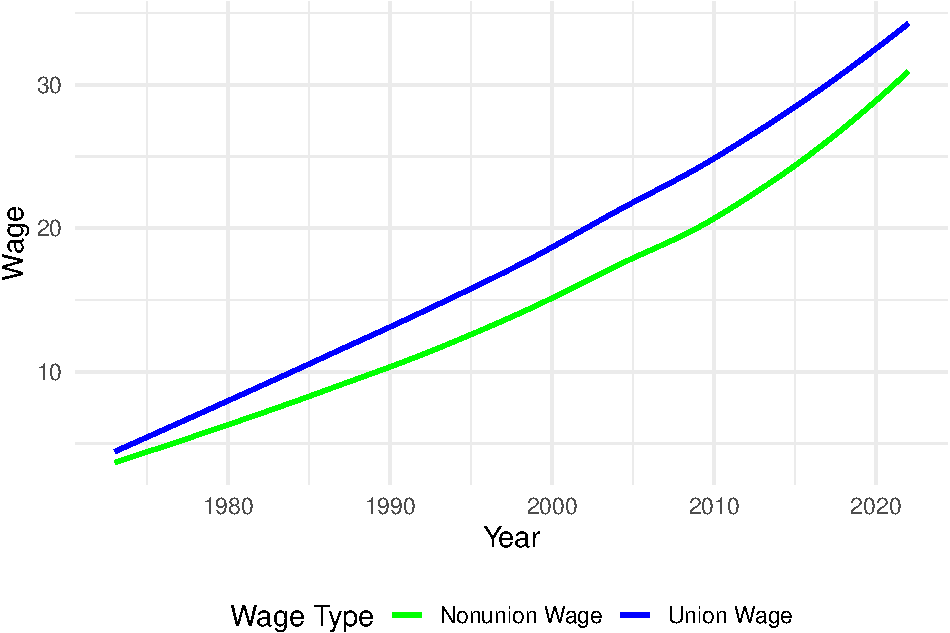
\includegraphics{_main_files/figure-latex/wagecomparison-1.pdf}
\caption{\label{fig:wagecomparison}Union Vs Non-Union Wages}
\end{figure}

As you can see the above code then creates a plot and places it in your document for you. This way you can fully customize the plot from within RStudio.

\subsection{Adding Images Using Markdown}\label{adding-images-using-markdown}

To add an image using Markdown, use the following syntax:

\begin{Shaded}
\begin{Highlighting}[]
\AlertTok{![Alt text for the image](images/drought{-}map.png)}
\end{Highlighting}
\end{Shaded}

\begin{itemize}
\tightlist
\item
  \textbf{Alt text}: A description of the image that is useful for accessibility.
\item
  \textbf{Path to the image}: This can be a relative path (e.g., ``) or a URL.
\end{itemize}

Example:

\begin{Shaded}
\begin{Highlighting}[]
\AlertTok{![A sample image](images/drought{-}map.png)}
\end{Highlighting}
\end{Shaded}

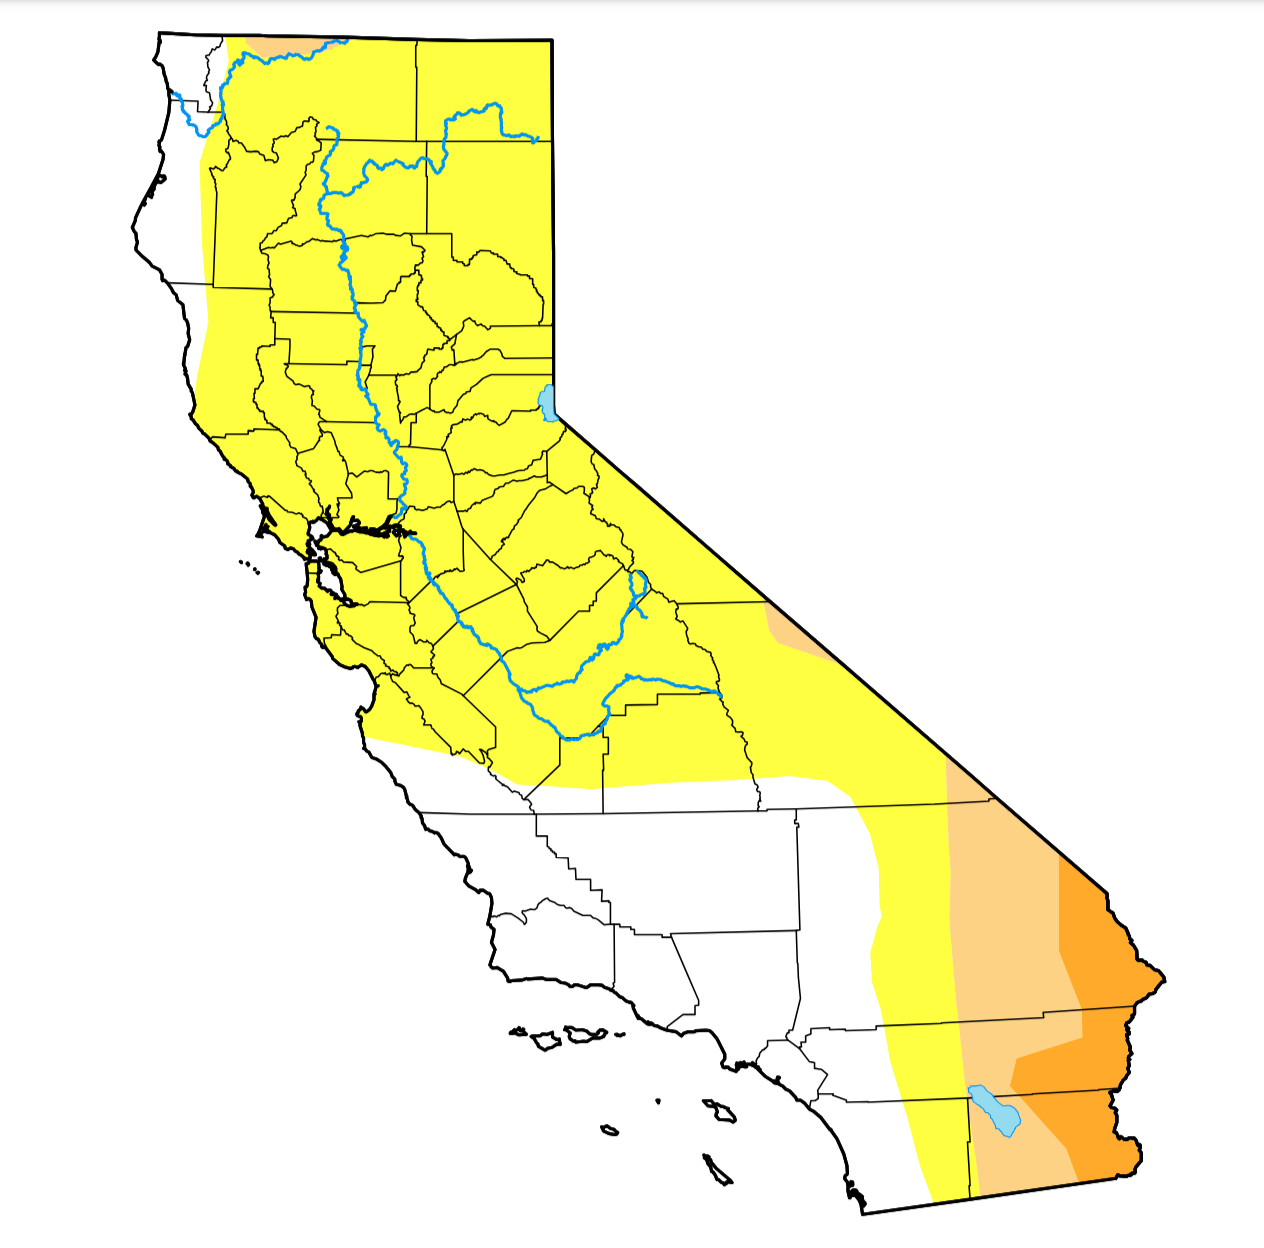
\includegraphics{images/drought-map.png}
\#\#\# Adding Images Using Code Chunks

You can also add images using an R code chunk, which can be useful when the image is generated programmatically. Use the \texttt{knitr::include\_graphics()} function:

\begin{Shaded}
\begin{Highlighting}[]
\NormalTok{knitr}\SpecialCharTok{::}\FunctionTok{include\_graphics}\NormalTok{(}\StringTok{"images/wageyear{-}1.png"}\NormalTok{)}
\end{Highlighting}
\end{Shaded}

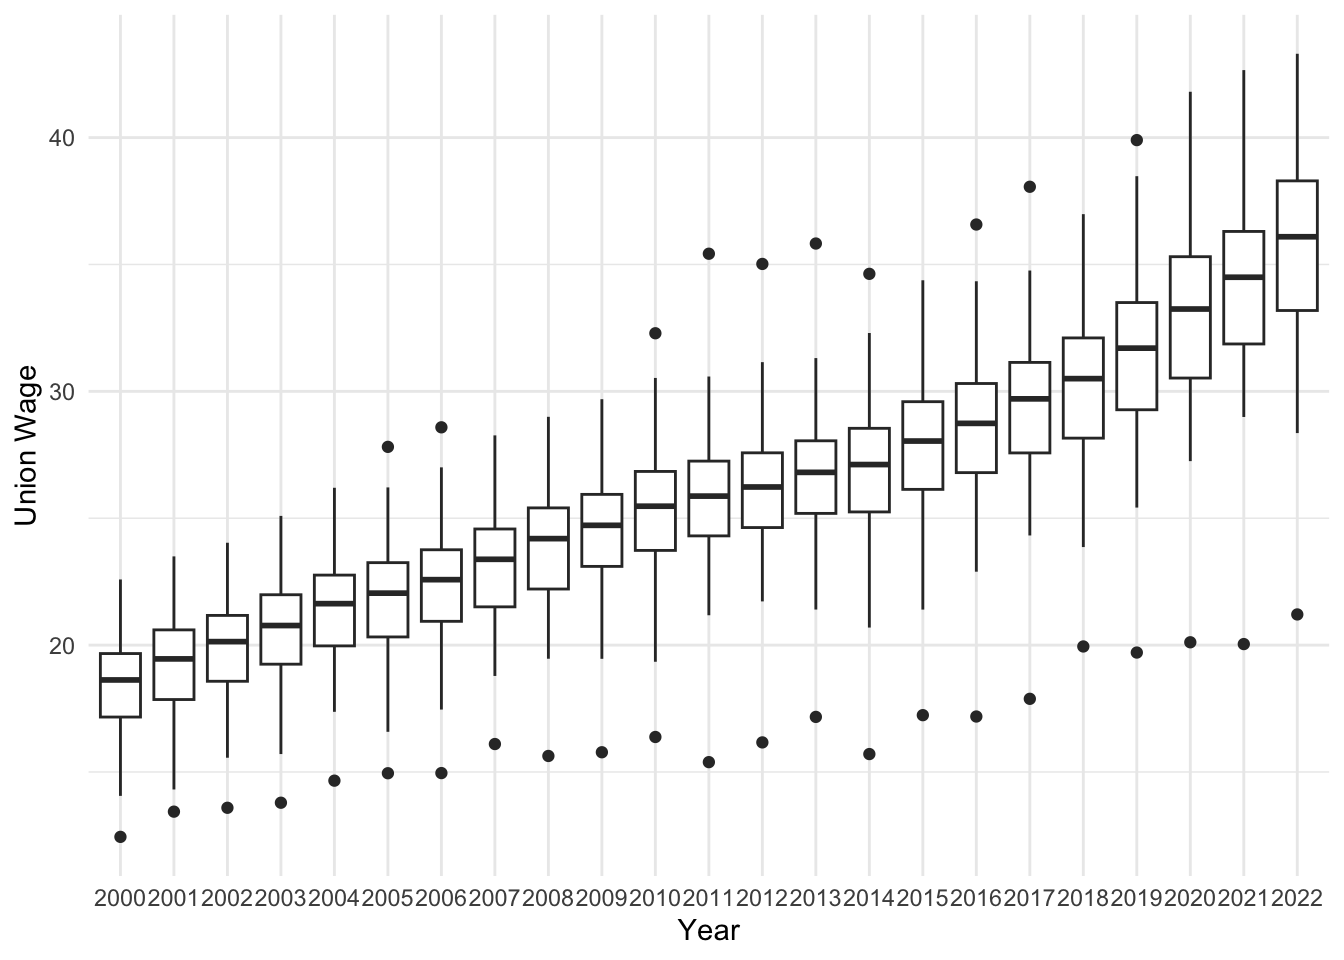
\includegraphics[width=18.67in]{images/wageyear-1}

\subsection{Chunk Options for Images}\label{chunk-options-for-images}

When adding images through code chunks, you can customize their appearance using chunk options such as \texttt{fig.cap} for captions and \texttt{out.width} for sizing.

For example the following has the caption \texttt{fig.cap="An\ example\ image"} and has an output width of 25\% with \texttt{out.width="25\%}. As you can see the image is much smaller than allowing the output width to not be adjusted.

\begin{Shaded}
\begin{Highlighting}[]
\NormalTok{knitr}\SpecialCharTok{::}\FunctionTok{include\_graphics}\NormalTok{(}\StringTok{"images/wageyear{-}1.png"}\NormalTok{)}
\end{Highlighting}
\end{Shaded}

\begin{figure}
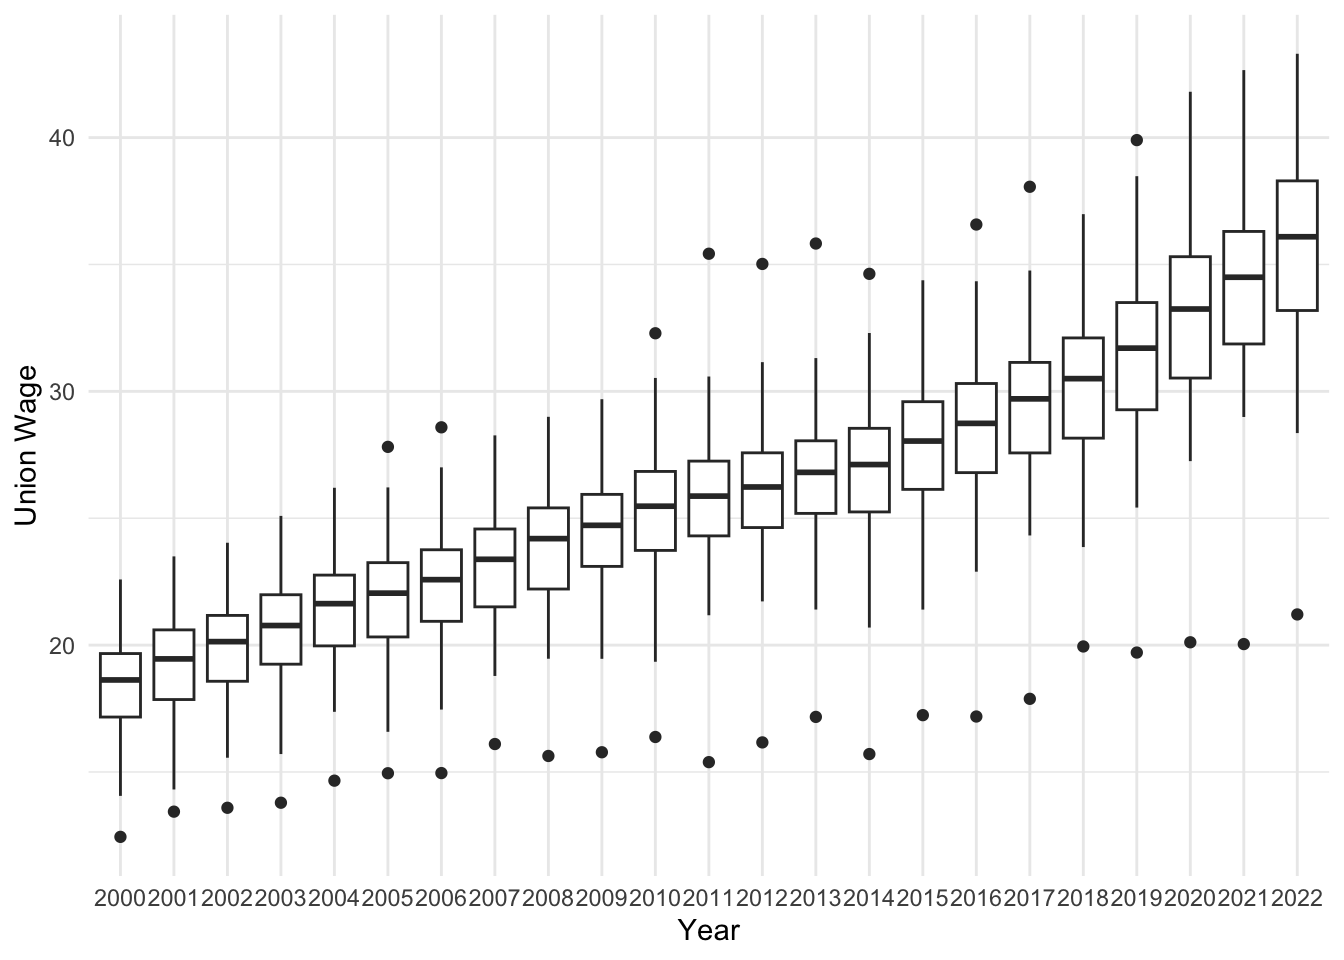
\includegraphics[width=0.25\linewidth]{images/wageyear-1} \caption{wageyear}\label{fig:unnamed-chunk-9}
\end{figure}

\begin{blackbox}

\begin{center}
\textbf{EXERCISE TIME!}

\end{center}

Create a new .Rmd file and write a short chapter that includes different types of Markdown elements (e.g., headers, lists, and images). Experiment with adding code chunks, andtext formatting.

\end{blackbox}

\chapter{Cross Referencing and Citatians}\label{chapter4}

Cross-references make it easier for readers to find and link to elements in your book. In Bookdown, you can create cross-references for sections, figures, tables, and equations. This chapter explains how to use cross-references effectively.

\begin{center}\rule{0.5\linewidth}{0.5pt}\end{center}

\section{Cross-Referencing Sections}\label{cross-referencing-sections}

To reference a section, first add an ID or tag to the heading by including \texttt{\{\#your-id\}} at the end of the section header. As an example here is the last chapter of the book that is an analysis I created within bookdown set as a single chapter:

\begin{Shaded}
\begin{Highlighting}[]
\FunctionTok{\# Example Document: Union Earnings Analysis (\#examplepaper)}
\end{Highlighting}
\end{Shaded}

You can then refer to it later, with a clickable link that will take your reader directly to it, in your document as follows:

\begin{Shaded}
\begin{Highlighting}[]
\NormalTok{See Section \textbackslash{}@ref(examplepaper) for more information.}
\end{Highlighting}
\end{Shaded}

\section{See Section \ref{examplepaper} for more information.}\label{see-section-refexamplepaper-for-more-information.}

\section{Cross-Referencing Text}\label{cross-referencing-text}

You can assign some text to a label and reference the text using the label elsewhere in your document. This can be particularly useful for long figure/table captions or when you need to reuse text fragments in multiple places.

The syntax for a text reference is \texttt{(ref:label)\ text}, where \texttt{label} is a unique label throughout the document. It must be in a separate paragraph with empty lines above and below it. The paragraph must not be wrapped into multiple lines, and should not end with whitespace.

\textbf{Additional Guidelines}:
- Ensure that text references are in a separate paragraph with empty lines above and below.
- Avoid wrapping the paragraph containing the text reference into multiple lines.
- Make sure there is no trailing whitespace at the end of the paragraph.

Example:

\begin{verbatim}



This is the text we are referencing
\end{verbatim} This is the text we are referencing

Then you can reference this text in your document using \texttt{(ref:textreference)}.

For example:

Then we reference it:
This is the text we are referencing
\end{verbatim}.

\begin{center}\rule{0.5\linewidth}{0.5pt}\end{center}

\section{Cross-Referencing Figures}\label{cross-referencing-figures}

To cross-reference a figure, set a chunk label and use the \texttt{fig.cap} option to add a caption. Bookdown automatically labels the figure with \texttt{fig:chunk-label}.

For example in the previous chapter we showed a plot comparing Union Wages vs Non-Union Wages. It had the following in the code chunk heading:

\texttt{\{r\ wagecomparison,\ fig.cap="Union\ Vs\ Non-Union\ Wages"\}}

We can easily create a reference back to this plot, that is clickable so users can easily go back to it, with the following:

\begin{Shaded}
\begin{Highlighting}[]
\NormalTok{See Figure \textbackslash{}@ref(fig:wagecomparison) for details.}
\end{Highlighting}
\end{Shaded}

See Figure \ref{fig:wagecomparison} for details.

\begin{center}\rule{0.5\linewidth}{0.5pt}\end{center}

\section{Cross-Referencing Tables}\label{cross-referencing-tables}

To cross-reference a table, use \texttt{knitr::kable()} to create a table with a caption. Bookdown automatically labels the table with \texttt{tab:chunk-label}.

Example:

\begin{Shaded}
\begin{Highlighting}[]
\NormalTok{knitr}\SpecialCharTok{::}\FunctionTok{kable}\NormalTok{(}\FunctionTok{head}\NormalTok{(cars), }\AttributeTok{caption =} \StringTok{"Table of the first rows of the cars dataset"}\NormalTok{)}
\end{Highlighting}
\end{Shaded}

\begin{table}

\caption{\label{tab:cars-table}Table of the first rows of the cars dataset}
\centering
\begin{tabular}[t]{r|r}
\hline
speed & dist\\
\hline
4 & 2\\
\hline
4 & 10\\
\hline
7 & 4\\
\hline
7 & 22\\
\hline
8 & 16\\
\hline
9 & 10\\
\hline
\end{tabular}
\end{table}

Reference this table using:

\begin{Shaded}
\begin{Highlighting}[]
\NormalTok{See Table \textbackslash{}@ref(tab:cars{-}table) for details.}
\end{Highlighting}
\end{Shaded}

See Table \ref{tab:cars-table} for details.

\begin{center}\rule{0.5\linewidth}{0.5pt}\end{center}

\section{Cross-Referencing Equations}\label{cross-referencing-equations}

For equations, use \texttt{(\textbackslash{}\#eq:label)} to label the equation and \texttt{\textbackslash{}@ref(eq:label)} to reference it. This way when you need to reference the equation at a later point in your document you can.

\subsection{Example: Creating and Labeling an Equation}\label{example-creating-and-labeling-an-equation}

First you write the equation in LaTeX in the equation environment and include the label as \texttt{(\textbackslash{}\#eq:label)}:

\begin{Shaded}
\begin{Highlighting}[]
\NormalTok{\textbackslash{}begin\{equation\}}
\NormalTok{  E = mc\^{}2}
\NormalTok{  (}\SpecialCharTok{\textbackslash{}\#}\NormalTok{eq:einstein)}
\NormalTok{\textbackslash{}end\{equation\}}
\end{Highlighting}
\end{Shaded}

Which outputs as such:

\begin{equation}
  E = mc^2
  \label{eq:einstein}
\end{equation}

Then at a later point when you need to reference it you simply type in \texttt{\textbackslash{}@ref(eq:label)}. As we know Einsten discovered that \eqref{eq:einstein}.

\section{Adding Citations and Managing References}\label{adding-citations-and-managing-references}

Bookdown makes it easy to manage references and add citations by using BibTeX files. Here's how to set up and include references in your Bookdown project.

\subsection{\texorpdfstring{Step 1: Create a \texttt{.bib} File}{Step 1: Create a .bib File}}\label{step-1-create-a-.bib-file}

First, create a \texttt{.bib} file for your references (e.g., \texttt{references.bib}). You can add references in BibTeX format. Here's an example entry:

\begin{Shaded}
\begin{Highlighting}[]
\VariableTok{@Book}\NormalTok{\{}\OtherTok{Bookdown}\NormalTok{,}
  \DataTypeTok{title}\NormalTok{     = \{Bookdown: Authoring Books and Technical Documents with R Markdown\},}
  \DataTypeTok{author}\NormalTok{    = \{Yihui Xie\},}
  \DataTypeTok{publisher}\NormalTok{ = \{Chapman; Hall/CRC\},}
  \DataTypeTok{year}\NormalTok{      = 2024,}
  \DataTypeTok{edition}\NormalTok{   = \{2nd\},}
  \DataTypeTok{note}\NormalTok{      = \{ISBN 9780367142568\},}
  \DataTypeTok{url}\NormalTok{       = \{https://bookdown.org/yihui/bookdown/\}}
\NormalTok{\}}
\end{Highlighting}
\end{Shaded}

\subsection{\texorpdfstring{Step 2: Link the \texttt{.bib} File in \texttt{index.Rmd}}{Step 2: Link the .bib File in index.Rmd}}\label{step-2-link-the-.bib-file-in-index.rmd}

In your \texttt{index.Rmd} file, include the \texttt{.bib} file in the YAML header:

\begin{Shaded}
\begin{Highlighting}[]
\AnnotationTok{bibliography:}\CommentTok{ [references.bib]}
\AnnotationTok{link{-}citations:}\CommentTok{ yes}
\end{Highlighting}
\end{Shaded}

\subsection{Step 3: Cite Sources in Your Text}\label{step-3-cite-sources-in-your-text}

To cite a source, use \texttt{{[}@citation-key{]}} in your text, where \texttt{citation-key} matches the key in your \texttt{.bib} file (e.g., \texttt{{[}@Bookdown{]}}). For example:

\begin{Shaded}
\begin{Highlighting}[]
\NormalTok{This tutorial was written thanks to Bookdown }\CommentTok{[}\OtherTok{@Bookdown}\CommentTok{]}\NormalTok{.}
\end{Highlighting}
\end{Shaded}

This tutorial was written thanks to Bookdown \citep{Bookdown}.

Bookdown will automatically format your citation based on the output style.

\subsection{Step 4: Customize Citation Style (Optional)}\label{step-4-customize-citation-style-optional}

If you need a specific citation style, you can add a \texttt{.csl} (Citation Style Language) file in your project and reference it in the YAML header:

\begin{Shaded}
\begin{Highlighting}[]
\AnnotationTok{csl:}\CommentTok{ "chicago{-}author{-}date.csl"}
\end{Highlighting}
\end{Shaded}

Download \texttt{.csl} files from sources like \href{https://www.zotero.org/styles}{Zotero}.

\section{Using Cross-References with Citations}\label{using-cross-references-with-citations}

In addition to referencing external sources, Bookdown allows you to cross-reference sections, figures, and tables, as discussed earlier. As a reminder:

\begin{Shaded}
\begin{Highlighting}[]
\NormalTok{As shown in Figure \textbackslash{}@ref(fig:example{-}figure), the trend is evident.}
\end{Highlighting}
\end{Shaded}

\section{Using cross-references with citations helps keep your document organized and easy to navigate.}\label{using-cross-references-with-citations-helps-keep-your-document-organized-and-easy-to-navigate.}

\begin{blackbox}

\begin{center}
\textbf{EXERCISE TIME!}

\end{center}

Go ahead and place a few entries in your .bib file. Once you've done that go through and reference these in your previously written content.

\end{blackbox}

\chapter{LaTeX in Bookdown}\label{chapter5}

Bookdown offers powerful support for LaTeX, allowing you to seamlessly integrate any LaTeX packages you need into your documents. Whether you're working with mathematical equations, theorems, lemmas, proofs, or other advanced features, this tutorial will guide you through the essentials of using LaTeX in Bookdown, showing you how to effectively incorporate and reference these elements.

\begin{center}\rule{0.5\linewidth}{0.5pt}\end{center}

\section{Including LaTeX Packages in Bookdown}\label{including-latex-packages-in-bookdown}

One of the powerful features of Bookdown is its seamless integration with LaTeX, allowing you to include any LaTeX package that suits your needs. This flexibility is especially useful when working with advanced mathematical notations, custom formatting, or specialized content.

\subsection{\texorpdfstring{Using a \texttt{preamble.tex} File}{Using a preamble.tex File}}\label{using-a-preamble.tex-file}

To include LaTeX packages, you need to create a \texttt{preamble.tex} file and link it in your \texttt{\_output.yml} file. The \texttt{preamble.tex} file is processed before the document is rendered allowing you to load any additional LaTeX packages you may need. The \texttt{preamble.tex} file also allows you to fully cuztomize the output of your PDF using your existing LaTeX knowledge.

\begin{enumerate}
\def\labelenumi{\arabic{enumi}.}
\tightlist
\item
  \textbf{Create a \texttt{preamble.tex} File}
  Create a file on your computer with the name \texttt{preamble.tex} and add it to the directory of your Bookdown project if it does not already exist. If the file already exists simply open the file within RStudi for easy editing. You can include as many packages as you need in the \texttt{preamble.tex} file. For example here is a list of packages and small changes I made to output the final example document in this tutorial as an a6 sized document:
\end{enumerate}

\begin{Shaded}
\begin{Highlighting}[]
\BuiltInTok{\textbackslash{}usepackage}\NormalTok{\{}\ExtensionTok{booktabs}\NormalTok{\}}
\BuiltInTok{\textbackslash{}usepackage}\NormalTok{\{}\ExtensionTok{anyfontsize}\NormalTok{\}}
\BuiltInTok{\textbackslash{}usepackage}\NormalTok{\{}\ExtensionTok{titlesec}\NormalTok{\}}
\BuiltInTok{\textbackslash{}usepackage}\NormalTok{\{}\ExtensionTok{fancyhdr}\NormalTok{\}}
\BuiltInTok{\textbackslash{}usepackage}\NormalTok{[paperwidth=4.13in, paperheight=5.83in]\{}\ExtensionTok{geometry}\NormalTok{\}}
\BuiltInTok{\textbackslash{}usepackage}\NormalTok{[font=small, labelfont=bf]\{}\ExtensionTok{caption}\NormalTok{\}}
\FunctionTok{\textbackslash{}geometry}\NormalTok{\{left=.5in\}}
\FunctionTok{\textbackslash{}geometry}\NormalTok{\{right=.5in\}}
\FunctionTok{\textbackslash{}geometry}\NormalTok{\{bottom=.5in\}}
\FunctionTok{\textbackslash{}geometry}\NormalTok{\{top=.75in\}}
\end{Highlighting}
\end{Shaded}

\begin{enumerate}
\def\labelenumi{\arabic{enumi}.}
\setcounter{enumi}{1}
\tightlist
\item
  \textbf{Link \texttt{preamble.tex} in \texttt{\_output.yml}}\\
  You need to make sure that the preamble is included in your \_output file. Update your \texttt{\_output.yml} file to include the \texttt{preamble.tex} file for PDF output:
\end{enumerate}

\begin{Shaded}
\begin{Highlighting}[]
\NormalTok{bookdown:}\SpecialCharTok{:pdf\_book:}
\NormalTok{  includes:}
\NormalTok{    in\_header: preamble.tex}
\NormalTok{  latex\_engine: xelatex}
\NormalTok{  citation\_package: natbib}
\NormalTok{  keep\_tex: yes}
\end{Highlighting}
\end{Shaded}

\subsection{Debugging Errors}\label{debugging-errors}

If your document fails to compile, check the error message in the console or look at the \texttt{.log} file generated by LaTeX for troubleshooting.

By including custom LaTeX packages, you can extend the functionality of your Bookdown project to suit your unique requirements, whether it's for academic papers, technical documents, or books.

\section{Mathematical Equations}\label{mathematical-equations}

Bookdown makes it easy to include both inline and display-style equations while also allowing you to reference these equations for easy reference at any point within your project.

\subsection{Inline Equations}\label{inline-equations}

Use \texttt{\$...\$} to include inline math equations within your text. The following code:

\begin{Shaded}
\begin{Highlighting}[]
\NormalTok{The formula for the area of a circle is $( A = \textbackslash{}pi r\^{}2 )$, where $( r )$ is the radius.}
\end{Highlighting}
\end{Shaded}

Then is displayed as follows:

The formula for the area of a circle is \(( A = \pi r^2 )\), where \(( r )\) is the radius.

\subsection{Display Equations}\label{display-equations}

For equations that you may want to have on their own line you have two options. You can surround your LaTeX code \texttt{\$\$...\$\$} or alternatively use the LaTeX \texttt{equation} environment.

Here we see the usage of \texttt{\$\$...\$\$}

\begin{Shaded}
\begin{Highlighting}[]
\NormalTok{$$}
\NormalTok{E = mc\^{}2}
\NormalTok{$$}
\end{Highlighting}
\end{Shaded}

Which gives us:

\[
E = mc^2
\]

Here we are using the \texttt{equation} environment with a label:

\begin{Shaded}
\begin{Highlighting}[]
\NormalTok{\textbackslash{}begin\{equation\}}
\NormalTok{  E = mc\^{}2}
\NormalTok{  (}\SpecialCharTok{\textbackslash{}\#}\NormalTok{eq:einstein)}
\NormalTok{\textbackslash{}end\{equation\}}
\end{Highlighting}
\end{Shaded}

Which outputs as such:

\begin{equation}
  E = mc^2
  \label{eq:einstein}
\end{equation}

Reminder for referencing equations: For easy reference within your document we are also able to add a reference to any equation by using \texttt{\textbackslash{}\#eq:your-label} as such:

\begin{verbatim}
\label{eq:einstein}
\end{verbatim}

So that you can easily reference it later with \texttt{\textbackslash{}@ref(eq:einstein)}. As an example, we labeled the above equation as \texttt{(\textbackslash{}\#eq:einstein)}. So we can reference it by using \texttt{\textbackslash{}@ref(eq:einstein)}:

\begin{Shaded}
\begin{Highlighting}[]
\NormalTok{As shown in Equation \textbackslash{}@ref(eq:einstein), energy is proportional to mass.}
\end{Highlighting}
\end{Shaded}

As shown in Equation \eqref{eq:einstein}, energy is proportional to mass.

\begin{center}\rule{0.5\linewidth}{0.5pt}\end{center}

\section{Theorems, Lemmas, and Proofs}\label{theorems-lemmas-and-proofs}

Bookdown supports theorems, lemmas, and proofs, for structured mathematical writing.

\subsection{Adding a Theorem}\label{adding-a-theorem}

Define a theorem using the following syntax:

\begin{Shaded}
\begin{Highlighting}[]
\NormalTok{::: \{.theorem \#theoremlabel\}}
\NormalTok{This is a }\InformationTok{\textasciigrave{}theorem\textasciigrave{}}\NormalTok{ environment that can contain **any**}
\NormalTok{\_Markdown\_ syntax.}
\NormalTok{For any integer $n \textbackslash{}geq 1$, the sum of the first $n$ positive integers is given by}
\NormalTok{$$}
\NormalTok{S = \textbackslash{}frac\{n(n + 1)\}\{2\}}
\NormalTok{$$}
\NormalTok{:::}
\end{Highlighting}
\end{Shaded}

Reference the theorem in your text by add \texttt{\#theoremlabel} to your code block as such:

\begin{Shaded}
\begin{Highlighting}[]
\NormalTok{::: \{.theorem \#theoremlabel\}}
\NormalTok{This is a }\InformationTok{\textasciigrave{}theorem\textasciigrave{}}\NormalTok{ environment that can contain **any**}
\NormalTok{\_Markdown\_ syntax.}
\NormalTok{For any integer $n \textbackslash{}geq 1$, the sum of the first $n$ positive integers is given by}
\NormalTok{$$}
\NormalTok{S = \textbackslash{}frac\{n(n + 1)\}\{2\}}
\NormalTok{$$}
\NormalTok{:::}
\end{Highlighting}
\end{Shaded}

Which will cause your theorem to display as follows:

\begin{theorem}
\protect\hypertarget{thm:theoremlabel}{}\label{thm:theoremlabel}This is a \texttt{theorem} environment that can contain \textbf{any}
\emph{Markdown} syntax.
For any integer \(n \geq 1\), the sum of the first \(n\) positive integers is given by
\[
S = \frac{n(n + 1)}{2}
\]
\end{theorem}

If this is a theorem that you need to reference in other parts of your document you can label it as we did above with \texttt{\#theoremlabel}. Then when you need to reference it you can do so using \texttt{\textbackslash{}@ref(thm:theoremlabel)} wherever needed. As an example, lets refer back to the above Theorem \ref{thm:theoremlabel}.

\subsection{Adding a Lemma}\label{adding-a-lemma}

Define a lemma similarly:

\begin{Shaded}
\begin{Highlighting}[]
\NormalTok{::: \{.lemma \#lemmalabel\}}
\NormalTok{Let $x\textbackslash{}in \textbackslash{}mathbb Z$.If $5x{-}7$ is odd,then $x$ is even.}
\NormalTok{:::}
\end{Highlighting}
\end{Shaded}

\begin{lemma}
\protect\hypertarget{lem:lemmalabel}{}\label{lem:lemmalabel}Let \(x \in \mathbb Z\). If \(5x-7\) is odd,then \(x\) is even.
\end{lemma}

Reference the lemma:

\begin{Shaded}
\begin{Highlighting}[]
\NormalTok{Lemma \textbackslash{}@ref(lem:lemmalabel) confirms that the sum of two even integers is even.}
\end{Highlighting}
\end{Shaded}

Lemma \ref{lem:lemmalabel} confirms that the sum of two even integers is even.

\subsection{Adding a Proof}\label{adding-a-proof}

Proofs can be added using the \texttt{proof} environment.

\begin{Shaded}
\begin{Highlighting}[]
\NormalTok{::: \{.proof\}}
\NormalTok{\textbackslash{}textbf\{Proof: \}Let $x \textbackslash{}in \textbackslash{}mathbb Z$. Suppose $7x+5$ is odd. Then $7x+5=2k+1$ for some $k \textbackslash{}in \textbackslash{}mathbb Z$. Then}
\NormalTok{\textbackslash{}begin\{align*\}}
\NormalTok{    7x+5\&=2k+1}\SpecialCharTok{\textbackslash{}\textbackslash{}}
\NormalTok{    7x\&=2k{-}4}\SpecialCharTok{\textbackslash{}\textbackslash{}}
\NormalTok{    x\&=2k{-}6x{-}4}\SpecialCharTok{\textbackslash{}\textbackslash{}}
\NormalTok{    x\&=2(k{-}3x{-}2).}
\NormalTok{\textbackslash{}end\{align*\}}
\NormalTok{Since $k{-}3x{-}2 \textbackslash{}in \textbackslash{}mathbb Z$, $x$ is even.}
\NormalTok{:::}
\end{Highlighting}
\end{Shaded}

\begin{proof}
\textbf{Proof: }Let \(x \in \mathbb Z\). Suppose \(7x+5\) is odd. Then \(7x+5=2k+1\) for some \(k \in \mathbb Z\). Then
\begin{align*}
    7x+5&=2k+1\\
    7x&=2k-4\\
    x&=2k-6x-4\\
    x&=2(k-3x-2).
\end{align*}
Since \(k-3x-2 \in \mathbb Z\), \(x\) is even.
\end{proof}

\begin{center}\rule{0.5\linewidth}{0.5pt}\end{center}

\subsection{Referencing Various Math Environments}\label{referencing-various-math-environments}

When you need to refer to create a different environment you just need to change what's between the brackets to the type of environment you are using.

\begin{Shaded}
\begin{Highlighting}[]
\NormalTok{::: \{.environment\}}
\NormalTok{Your information goes here}
\NormalTok{:::}
\end{Highlighting}
\end{Shaded}

When you are referencing the environment you would just ensure that you use the label prefix from the below table for the environment you wish to reference, changing the word prefix in:\texttt{\textbackslash{}@ref(prefix:label)} to the appropriate environment.

\begin{table}

\caption{\label{tab:theorem-table}Theorem environments in Bookdown.}
\centering
\begin{tabular}[t]{lll}
\toprule
Environment & Printed Name & Label Prefix\\
\midrule
theorem & Theorem & thm\\
lemma & Lemma & lem\\
corollary & Corollary & cor\\
proposition & Proposition & prp\\
conjecture & Conjecture & cnj\\
\addlinespace
definition & Definition & def\\
example & Example & exm\\
exercise & Exercise & exr\\
hypothesis & Hypothesis & hyp\\
\bottomrule
\end{tabular}
\end{table}

\section{Tips for LaTeX in Bookdown}\label{tips-for-latex-in-bookdown}

\begin{itemize}
\tightlist
\item
  \textbf{Use Labels Consistently}: Use meaningful and unique labels for cross-referencing.
\item
  \textbf{Use Math Mode}: Always enclose mathematical symbols in \texttt{\$...\$} or \texttt{\$\$...\$\$} to render correctly.
\item
  \textbf{Add Theorem Styles}: Customize theorem environments in \texttt{\_bookdown.yml} for specific needs:
  \texttt{markdown\ \ theorem:\ \ \ \ lab:\ "Theorem\ "\ \ \ \ lem:\ "Lemma\ "}
\end{itemize}

\begin{blackbox}

\begin{center}
\textbf{EXERCISE TIME!}

\end{center}

Add an equation and a theorem to your document using LaTeX. Alternatively, copy over some LaTeX code you've written before and place it in one of your chapters.

\end{blackbox}

\chapter{Advanced Features}\label{chapter6}

In this chapter, we'll explore some advanced features of Bookdown.

\begin{center}\rule{0.5\linewidth}{0.5pt}\end{center}

\section{Using LaTeX for Advanced Formatting}\label{using-latex-for-advanced-formatting}

Bookdown supports advanced formatting using \textbf{LaTeX}. This allows you to create custom environments, add annotations, and format mathematical content beautifully.

\subsection{Example: Adding a Custom Box}\label{example-adding-a-custom-box}

You can define a custom LaTeX environment for a ``black note box'' in the \texttt{preamble.tex} file:

\begin{Shaded}
\begin{Highlighting}[]
\FunctionTok{\textbackslash{}setlength}\NormalTok{\{}\FunctionTok{\textbackslash{}fboxsep}\NormalTok{\}\{.8em\}}

\FunctionTok{\textbackslash{}newenvironment}\NormalTok{\{blackbox\}\{}
  \FunctionTok{\textbackslash{}definecolor}\NormalTok{\{shadecolor\}\{rgb\}\{0, 0, 0\}  }\CommentTok{\% black}
  \FunctionTok{\textbackslash{}color}\NormalTok{\{white\}}
  \KeywordTok{\textbackslash{}begin}\NormalTok{\{}\ExtensionTok{shaded}\NormalTok{\}\}}
\NormalTok{ \{}\KeywordTok{\textbackslash{}end}\NormalTok{\{}\ExtensionTok{shaded}\NormalTok{\}\}}
\end{Highlighting}
\end{Shaded}

Then use the custom box in your content:

\begin{Shaded}
\begin{Highlighting}[]
\NormalTok{:::: \{.blackbox data{-}latex=""\}}
\NormalTok{::: \{.center data{-}latex=""\}}
\NormalTok{**EXAMPLE!**}
\NormalTok{:::}
\NormalTok{Giving you this as an output.}
\NormalTok{::::}
\end{Highlighting}
\end{Shaded}

\begin{blackbox}

\begin{center}
\textbf{EXAMPLE!}

\end{center}

Giving you this as an output.

\end{blackbox}

\begin{center}\rule{0.5\linewidth}{0.5pt}\end{center}

\section{Customizing Document with LaTeX}\label{customizing-document-with-latex}

You can even customize the entire look and output of your document by editing the content in your preamble. For example, say you wish to create an a6 size booklet and so need to modify the font sizes as I did in the for the Example Document at the end of this tutorial. In thise the preamble would look as follows:

\begin{Shaded}
\begin{Highlighting}[]
\NormalTok{\textbackslash{}usepackage\{booktabs\}}
\NormalTok{\textbackslash{}usepackage\{anyfontsize\}}
\NormalTok{\textbackslash{}usepackage\{titlesec\}}
\NormalTok{\textbackslash{}usepackage\{fancyhdr\}}
\NormalTok{\textbackslash{}usepackage}\CommentTok{[}\OtherTok{paperwidth=4.13in, paperheight=5.83in}\CommentTok{]}\NormalTok{\{geometry\}}
\NormalTok{\textbackslash{}usepackage}\CommentTok{[}\OtherTok{font=small, labelfont=bf}\CommentTok{]}\NormalTok{\{caption\}}
\NormalTok{\textbackslash{}geometry\{left=.5in\}}
\NormalTok{\textbackslash{}geometry\{right=.5in\}}
\NormalTok{\textbackslash{}geometry\{bottom=.5in\}}
\NormalTok{\textbackslash{}geometry\{top=.75in\}}
\NormalTok{\textbackslash{}renewcommand\{\textbackslash{}normalsize\}\{\textbackslash{}fontsize\{6pt\}\{8pt\}\textbackslash{}selectfont\}}
\NormalTok{\textbackslash{}titleformat\{\textbackslash{}section\}\{\textbackslash{}fontsize\{8pt\}\{10pt\}\textbackslash{}bfseries\}\{\textbackslash{}thesection\}\{1em\}\{\}}
\NormalTok{\textbackslash{}titleformat\{\textbackslash{}subsection\}\{\textbackslash{}fontsize\{6pt\}\{8pt\}\textbackslash{}bfseries\}\{\textbackslash{}thesubsection\}\{1em\}\{\}}
\NormalTok{\textbackslash{}titleformat\{\textbackslash{}subsubsection\}\{\textbackslash{}fontsize\{7pt\}\{9pt\}\textbackslash{}bfseries\}\{\textbackslash{}thesubsubsection\}\{1em\}\{\}}
\NormalTok{\textbackslash{}usepackage\{tocloft\}}
\NormalTok{\textbackslash{}renewcommand\{\textbackslash{}cftsecfont\}\{\textbackslash{}fontsize\{6pt\}\{8pt\}\}}
\NormalTok{\textbackslash{}renewcommand\{\textbackslash{}cftsubsecfont\}\{\textbackslash{}fontsize\{7pt\}\{9pt\}\}}
\NormalTok{\textbackslash{}renewcommand\{\textbackslash{}cftsubsubsecfont\}\{\textbackslash{}fontsize\{6pt\}\{8pt\}\}}
\NormalTok{\textbackslash{}usepackage\{listings\}}
\NormalTok{\textbackslash{}lstset\{}
\NormalTok{  basicstyle=\textbackslash{}ttfamily\textbackslash{}fontsize\{2pt\}\{4pt\},}
\NormalTok{  breaklines=false,}
\NormalTok{  frame=single,}
\NormalTok{\}}
\NormalTok{\textbackslash{}usepackage\{titlesec\}}
\NormalTok{\textbackslash{}titleformat\{\textbackslash{}chapter\}}\CommentTok{[}\OtherTok{display}\CommentTok{]}
\NormalTok{  \{\textbackslash{}fontsize\{14pt\}\{18pt\}\textbackslash{}bfseries\} }
\NormalTok{  \{\textbackslash{}chaptername\textasciitilde{}\textbackslash{}thechapter\}       }
\NormalTok{  \{1em\}                            }
\NormalTok{  \{\}}
\NormalTok{\textbackslash{}titleformat\{\textbackslash{}section\}}
\NormalTok{  \{\textbackslash{}fontsize\{10pt\}\{12pt\}\textbackslash{}bfseries\} }
\NormalTok{  \{\textbackslash{}thesection\}                    }
\NormalTok{  \{1em\}                            }
\NormalTok{  \{\}}
\NormalTok{\textbackslash{}titleformat\{\textbackslash{}subsection\}}
\NormalTok{  \{\textbackslash{}fontsize\{10pt\}\{12pt\}\textbackslash{}bfseries\} }
\NormalTok{  \{\textbackslash{}thesubsection\}                 }
\NormalTok{  \{1em\}                            }
\NormalTok{  \{\}}
\NormalTok{\textbackslash{}setlength\{\textbackslash{}fboxsep\}\{.8em\}}
\end{Highlighting}
\end{Shaded}

\section{Adding Custom CSS and JavaScript}\label{adding-custom-css-and-javascript}

Enhance the appearance and functionality of your Bookdown project by adding custom CSS and JavaScript.

\subsection{Step 1: Create a Custom CSS File}\label{step-1-create-a-custom-css-file}

Create a \texttt{styles.css} file with your custom styles:

\begin{Shaded}
\begin{Highlighting}[]
\NormalTok{body \{}
  \KeywordTok{font{-}family}\CharTok{:} \StringTok{"Arial"}\OperatorTok{,} \DecValTok{sans{-}serif}\OperatorTok{;}
\NormalTok{\}}
\NormalTok{h1 \{}
  \KeywordTok{color}\CharTok{:} \ConstantTok{\#4CAF50}\OperatorTok{;}
\NormalTok{\}}
\end{Highlighting}
\end{Shaded}

\subsection{Step 2: Include the CSS File in the YAML Header}\label{step-2-include-the-css-file-in-the-yaml-header}

Add the following to your \texttt{index.Rmd}:

\begin{Shaded}
\begin{Highlighting}[]
\AnnotationTok{output:}
\NormalTok{  bookdown:}\SpecialCharTok{:gitbook:}
\NormalTok{    css: styles.css}
\end{Highlighting}
\end{Shaded}

\subsection{Step 3: Adding JavaScript (Optional)}\label{step-3-adding-javascript-optional}

For dynamic behavior, include JavaScript files similarly:

\begin{Shaded}
\begin{Highlighting}[]
\AnnotationTok{output:}
\NormalTok{  bookdown:}\SpecialCharTok{:gitbook:}
\NormalTok{    includes:}
\NormalTok{      in\_header: "scripts.js"}
\end{Highlighting}
\end{Shaded}

\begin{blackbox}

\begin{center}
\textbf{EXERCISE TIME!}

\end{center}

Use custom LaTeX to add a unique visual element to your content (e.g., a shaded box or note). Play around with the settings and see what you like best.

\end{blackbox}

\chapter{Customizing Output}\label{chapter7}

In this chapter, we'll explore how to customize the output of your Bookdown project. Bookdown supports several output formats, such as HTML, PDF, and EPUB, and allows you to customize each format to match your project's needs. We'll cover choosing output formats, modifying appearance, and configuring output settings.

\begin{center}\rule{0.5\linewidth}{0.5pt}\end{center}

\section{Choosing an Output Format}\label{choosing-an-output-format}

Bookdown provides multiple output formats that allow you to publish your document in various ways:

\begin{itemize}
\tightlist
\item
  \textbf{HTML}: Ideal for online documentation or sharing on the web.
\item
  \textbf{PDF}: Useful for print-ready documents, especially for academic or professional reports.
\item
  \textbf{EPUB}: E-book format, compatible with e-readers for mobile access.
\end{itemize}

To specify output formats, edit the \texttt{\_output.yml} file in your project directory. Here's an example configuration:

\begin{Shaded}
\begin{Highlighting}[]
\NormalTok{bookdown:}\SpecialCharTok{:gitbook:}
\NormalTok{  css: "style.css"}
\NormalTok{  split\_by: "chapter"}

\NormalTok{bookdown:}\SpecialCharTok{:pdf\_book:}
\NormalTok{  latex\_engine: xelatex}
\NormalTok{  citation\_package: natbib}

\NormalTok{bookdown:}\SpecialCharTok{:epub\_book:}\NormalTok{ default}
\end{Highlighting}
\end{Shaded}

This configuration tells Bookdown to create HTML (using GitBook style), PDF, and EPUB formats. Customize each format's settings to control the output style.

\begin{center}\rule{0.5\linewidth}{0.5pt}\end{center}

\section{Available Output Options for Bookdown}\label{available-output-options-for-bookdown}

\subsection{\texorpdfstring{1. GitBook (\texttt{bookdown::gitbook})}{1. GitBook (bookdown::gitbook)}}\label{gitbook-bookdowngitbook}

This is one of the most popular output formats, producing an HTML book with interactive features such as search and navigation. Infact this is how the book has been outputted.

Example:

\begin{Shaded}
\begin{Highlighting}[]
\AnnotationTok{output:}
\NormalTok{  bookdown:}\SpecialCharTok{:gitbook:}
\NormalTok{    css: style.css  \# Optional: Custom CSS for styling}
\NormalTok{    config:}
\NormalTok{      toc:}
\NormalTok{        collapse: section  \# Controls the collapsing of the table of contents}
\end{Highlighting}
\end{Shaded}

\subsection{\texorpdfstring{2. PDF Book (\texttt{bookdown::pdf\_book})}{2. PDF Book (bookdown::pdf\_book)}}\label{pdf-book-bookdownpdf_book}

Generates a PDF version of your book using LaTeX. This format is often used for printed versions.

Example:

\begin{Shaded}
\begin{Highlighting}[]
\AnnotationTok{output:}
\NormalTok{  bookdown:}\SpecialCharTok{:pdf\_book:}
\NormalTok{    latex\_engine: xelatex  \# Specify the LaTeX engine to use (e.g., pdflatex, xelatex, lualatex)}
\NormalTok{    includes:}
\NormalTok{      in\_header: preamble.tex  \# Include additional LaTeX setup files}
\NormalTok{    citation\_package: natbib  \# Citation package to use}
\end{Highlighting}
\end{Shaded}

\subsection{\texorpdfstring{3. EPUB Book (\texttt{bookdown::epub\_book})}{3. EPUB Book (bookdown::epub\_book)}}\label{epub-book-bookdownepub_book}

Creates an EPUB file, which is a format commonly used for eBooks.

Example:

\begin{Shaded}
\begin{Highlighting}[]
\AnnotationTok{output:}
\NormalTok{  bookdown:}\SpecialCharTok{:epub\_book:}
\NormalTok{    toc: yes  \# Include table of contents}
\NormalTok{    css: style.css  \# Optional: Custom CSS for EPUB styling}
\end{Highlighting}
\end{Shaded}

\subsection{\texorpdfstring{4. HTML Document (\texttt{rmarkdown::html\_document})}{4. HTML Document (rmarkdown::html\_document)}}\label{html-document-rmarkdownhtml_document}

Produces a single HTML document, rather than a book format.

Example:

\begin{Shaded}
\begin{Highlighting}[]
\AnnotationTok{output:}
\NormalTok{  rmarkdown:}\SpecialCharTok{:html\_document:}
\NormalTok{    toc: true  \# Include table of contents}
\NormalTok{    toc\_depth: 3  \# Depth of the table of contents}
\NormalTok{    number\_sections: true  \# Number sections in the output}
\end{Highlighting}
\end{Shaded}

\subsection{\texorpdfstring{5. Word Document (\texttt{bookdown::word\_document2})}{5. Word Document (bookdown::word\_document2)}}\label{word-document-bookdownword_document2}

Generates a Word document (\texttt{.docx}) version of your book, useful for sharing with editors.

Example:

\begin{Shaded}
\begin{Highlighting}[]
\AnnotationTok{output:}
\NormalTok{  bookdown:}\SpecialCharTok{:word\_document2:}
\NormalTok{    toc: yes  \# Include table of contents}
\NormalTok{    toc\_depth: 2  \# Depth of table of contents}
\end{Highlighting}
\end{Shaded}

\subsection{\texorpdfstring{6. Tufte Handout (\texttt{bookdown::tufte\_html\_book} / \texttt{bookdown::tufte\_pdf\_book})}{6. Tufte Handout (bookdown::tufte\_html\_book / bookdown::tufte\_pdf\_book)}}\label{tufte-handout-bookdowntufte_html_book-bookdowntufte_pdf_book}

Generates a book in Tufte style, known for its distinctive design, which is suitable for visually focused content.

Example:

\begin{Shaded}
\begin{Highlighting}[]
\AnnotationTok{output:}
\NormalTok{  bookdown:}\SpecialCharTok{:tufte\_html\_book:}\NormalTok{ default}
\end{Highlighting}
\end{Shaded}

For PDF:

\begin{Shaded}
\begin{Highlighting}[]
\AnnotationTok{output:}
\NormalTok{  bookdown:}\SpecialCharTok{:tufte\_pdf\_book:}\NormalTok{ default}
\end{Highlighting}
\end{Shaded}

\subsection{\texorpdfstring{7. HTML with Bookdown-Specific Features (\texttt{bookdown::html\_document2})}{7. HTML with Bookdown-Specific Features (bookdown::html\_document2)}}\label{html-with-bookdown-specific-features-bookdownhtml_document2}

Similar to \texttt{rmarkdown::html\_document} but includes additional cross-referencing features from Bookdown.

Example:

\begin{Shaded}
\begin{Highlighting}[]
\AnnotationTok{output:}
\NormalTok{  bookdown:}\SpecialCharTok{:html\_document2:}
\NormalTok{    toc: true}
\NormalTok{    number\_sections: true}
\end{Highlighting}
\end{Shaded}

\subsection{\texorpdfstring{8. GitHub Document (\texttt{rmarkdown::github\_document})}{8. GitHub Document (rmarkdown::github\_document)}}\label{github-document-rmarkdowngithub_document}

Produces a document suitable for rendering on GitHub.

Example:

\begin{Shaded}
\begin{Highlighting}[]
\AnnotationTok{output:}
\NormalTok{  rmarkdown:}\SpecialCharTok{:github\_document:}
\NormalTok{    toc: true  \# Include table of contents}
\end{Highlighting}
\end{Shaded}

\begin{center}\rule{0.5\linewidth}{0.5pt}\end{center}

\section{Customizing HTML Output}\label{customizing-html-output}

To customize the HTML format, Bookdown offers the \texttt{bookdown::gitbook} and \texttt{bookdown::html\_document2} options:

\begin{itemize}
\tightlist
\item
  \textbf{GitBook}: The default HTML style, which includes a side navigation bar and a search function. This format is ideal for online documentation.
\item
  \textbf{HTML Document}: A simpler format without the sidebar, suitable for single-page reports.
\end{itemize}

You can adjust HTML settings in \texttt{\_output.yml}:

\begin{Shaded}
\begin{Highlighting}[]
\NormalTok{bookdown:}\SpecialCharTok{:gitbook:}
\NormalTok{  css: "style.css"}
\NormalTok{  config:}
\NormalTok{    toc:}
\NormalTok{      collapse: section}
\NormalTok{    download: }\CommentTok{[}\OtherTok{"pdf", "epub"}\CommentTok{]}
\end{Highlighting}
\end{Shaded}

\begin{center}\rule{0.5\linewidth}{0.5pt}\end{center}

\section{Customizing PDF Output}\label{customizing-pdf-output}

To generate a high-quality PDF, you'll need to install a LaTeX distribution like TinyTeX.

In \texttt{\_output.yml}, you can specify options to control PDF formatting:

\begin{Shaded}
\begin{Highlighting}[]
\NormalTok{bookdown:}\SpecialCharTok{:pdf\_book:}
\NormalTok{  latex\_engine: xelatex}
\NormalTok{  citation\_package: natbib}
\end{Highlighting}
\end{Shaded}

\begin{itemize}
\tightlist
\item
  \textbf{\texttt{latex\_engine}}: Specifies the LaTeX engine (e.g., \texttt{xelatex}, \texttt{pdflatex}). Using \texttt{xelatex} improves font compatibility.
\item
  \textbf{\texttt{citation\_package}}: Choose between \texttt{natbib} or \texttt{biblatex} for handling citations.
\end{itemize}

\subsection{Document Size}\label{document-size}

To customize the size of your PDF document, you can modify the \texttt{geometry} option in the LaTeX preamble. For example, to set the paper size to A4 and customize the margins:

\begin{Shaded}
\begin{Highlighting}[]
\AnnotationTok{output:}
\NormalTok{  bookdown:}\SpecialCharTok{:pdf\_book:}
\NormalTok{    includes:}
\NormalTok{      in\_header: preamble.tex}
\end{Highlighting}
\end{Shaded}

In the \texttt{preamble.tex} file, add:

\begin{Shaded}
\begin{Highlighting}[]
\NormalTok{\textbackslash{}usepackage}\CommentTok{[}\OtherTok{paperwidth=5.5in, paperheight=8.5in, margin=0.75in}\CommentTok{]}\NormalTok{\{geometry\}}
\end{Highlighting}
\end{Shaded}

This sets the document size to A4 and the margins to 1 inch.

\subsection{Document Type}\label{document-type}

You can change the document type by modifying the LaTeX class used in the \texttt{preamble.tex}. For example, use the \texttt{article} class instead of the default \texttt{book} class:

\begin{Shaded}
\begin{Highlighting}[]
\NormalTok{\textbackslash{}documentclass\{article\}}
\end{Highlighting}
\end{Shaded}

This is useful for a more compact layout, like that of a research paper or report.

\subsection{LaTeX Engine}\label{latex-engine}

You can specify the LaTeX engine used to compile your PDF. Bookdown supports different engines, such as \texttt{pdflatex}, \texttt{xelatex}, and \texttt{lualatex}.

Example:

\begin{Shaded}
\begin{Highlighting}[]
\AnnotationTok{output:}
\NormalTok{  bookdown:}\SpecialCharTok{:pdf\_book:}
\NormalTok{    latex\_engine: xelatex}
\end{Highlighting}
\end{Shaded}

Using \texttt{xelatex} or \texttt{lualatex} provides better font support, especially for special characters or non-Latin scripts.

\subsection{Custom LaTeX Packages}\label{custom-latex-packages}

Include custom LaTeX packages in the \texttt{preamble.tex} file to extend the functionality of your PDF output.

Example:

\begin{Shaded}
\begin{Highlighting}[]
\BuiltInTok{\textbackslash{}usepackage}\NormalTok{\{}\ExtensionTok{amsmath}\NormalTok{\}}
\end{Highlighting}
\end{Shaded}

This includes the \texttt{amsmath} package for advanced mathematical formatting. You can also use \texttt{\textbackslash{}newcommand} to define custom commands used throughout your document.

\subsection{Page Layout Customization}\label{page-layout-customization}

To customize the page layout, use packages like \texttt{fancyhdr} to modify headers and footers.

Example:

\begin{Shaded}
\begin{Highlighting}[]
\BuiltInTok{\textbackslash{}usepackage}\NormalTok{\{}\ExtensionTok{fancyhdr}\NormalTok{\}}
\FunctionTok{\textbackslash{}pagestyle}\NormalTok{\{fancy\}}
\FunctionTok{\textbackslash{}fancyhead}\NormalTok{[LE,RO]\{Your Book Title\}}
\FunctionTok{\textbackslash{}fancyfoot}\NormalTok{[CE,CO]\{}\FunctionTok{\textbackslash{}thepage}\NormalTok{\}}
\end{Highlighting}
\end{Shaded}

This sets custom headers and footers, including the book title and page numbers.

\begin{center}\rule{0.5\linewidth}{0.5pt}\end{center}

\section{Customizing EPUB Output}\label{customizing-epub-output}

To create an EPUB e-book, use \texttt{bookdown::epub\_book} in \texttt{\_output.yml}. Bookdown handles most EPUB formatting automatically, but you can make some modifications:

\begin{Shaded}
\begin{Highlighting}[]
\NormalTok{bookdown:}\SpecialCharTok{:epub\_book:}
\NormalTok{  stylesheet: "style.css"}
\NormalTok{  cover\_image: "images/cover.jpg"}
\NormalTok{  toc: yes}
\end{Highlighting}
\end{Shaded}

This configuration adds a cover image, applies the CSS stylesheet, and includes a table of contents.

\begin{center}\rule{0.5\linewidth}{0.5pt}\end{center}

\section{\texorpdfstring{Specifying Global Settings in \texttt{\_bookdown.yml}}{Specifying Global Settings in \_bookdown.yml}}\label{specifying-global-settings-in-_bookdown.yml}

The \texttt{\_bookdown.yml} file allows you to set global configurations, such as the order of chapters, the naming convention for output files, and the label format for figures and tables. Here's an example:

\begin{Shaded}
\begin{Highlighting}[]
\AnnotationTok{book\_filename:}\CommentTok{ "my{-}book"}
\AnnotationTok{rmd\_files:}\CommentTok{ ["index.Rmd", "01{-}introduction.Rmd", "02{-}writing{-}structuring{-}content.Rmd", "03{-}customizing{-}output.Rmd"]}
\AnnotationTok{language:}
\NormalTok{  label:}
\NormalTok{    fig: "Figure "}
\NormalTok{    tab: "Table "}
\NormalTok{delete\_merged\_file: true}
\end{Highlighting}
\end{Shaded}

\begin{itemize}
\tightlist
\item
  \textbf{\texttt{book\_filename}}: Sets the base filename for output files.
\item
  \textbf{\texttt{rmd\_files}}: Specifies the order of chapters.
\item
  \textbf{\texttt{language.label}}: Customizes labels for figures and tables.
\item
  \textbf{\texttt{delete\_merged\_file}}: Deletes intermediary files after rendering, keeping the directory clean.
\end{itemize}

\begin{center}\rule{0.5\linewidth}{0.5pt}\end{center}

\section{Example Output}\label{example-output}

To render all formats simultaneously, you can use the \texttt{render\_book()} function in the R console:

\begin{Shaded}
\begin{Highlighting}[]
\NormalTok{bookdown}\SpecialCharTok{::}\FunctionTok{render\_book}\NormalTok{(}\StringTok{"index.Rmd"}\NormalTok{, }\AttributeTok{output\_format =} \StringTok{"all"}\NormalTok{)}
\end{Highlighting}
\end{Shaded}

This command generates HTML, PDF, and EPUB files as specified in \texttt{\_output.yml}.

\begin{blackbox}

\begin{center}
\textbf{EXERCISE TIME!}

\end{center}

Modify your Bookdown project's \_output.yml to customize the output format. Try changing the appearance of the HTML and PDF outputs. Write a paragraph explaining how the customizations improved the document's look and usability.

When you're ready go ahead and render your book into HTML, PDF, and EPUB formats. Publish it on GitHub Pages or share it with someone else. Write a paragraph reflecting on what you learned about the publishing process and any challenges you encountered.

\end{blackbox}

\chapter{LaTeX Distributions}\label{latexdistributions}

To render PDF outputs with Bookdown, you need to install a LaTeX distribution. Below is a list of popular options, categorized by operating system and user preferences:

\section{Recommended LaTeX Distribution}\label{recommended-latex-distribution}

\subsection{\texorpdfstring{1. \textbf{TinyTeX} (Recommended)}{1. TinyTeX (Recommended)}}\label{tinytex-recommended}

\begin{itemize}
\item
  \textbf{Description}: A lightweight, cross-platform LaTeX distribution designed to work seamlessly with R and Bookdown.
\item
  \textbf{Installation}: Run the following commands in R:

\begin{Shaded}
\begin{Highlighting}[]
\FunctionTok{install.packages}\NormalTok{(}\StringTok{"tinytex"}\NormalTok{)}
\NormalTok{tinytex}\SpecialCharTok{::}\FunctionTok{install\_tinytex}\NormalTok{()}
\end{Highlighting}
\end{Shaded}
\item
  \textbf{Advantages}:

  \begin{itemize}
  \tightlist
  \item
    Minimal installation size.
  \item
    Automatically installs missing packages when rendering.
  \end{itemize}
\item
  \textbf{Website}: \href{https://yihui.org/tinytex/}{TinyTeX Documentation}
\end{itemize}

\begin{center}\rule{0.5\linewidth}{0.5pt}\end{center}

\section{Additional LaTeX Distributions}\label{additional-latex-distributions}

\subsection{\texorpdfstring{2. \textbf{TeX Live}}{2. TeX Live}}\label{tex-live}

\begin{itemize}
\tightlist
\item
  \textbf{Description}: A comprehensive LaTeX distribution suitable for Linux and cross-platform users.
\item
  \textbf{Installation}:

  \begin{itemize}
  \item
    \textbf{Linux}:

\begin{Shaded}
\begin{Highlighting}[]
\FunctionTok{sudo}\NormalTok{ apt{-}get install texlive{-}full}
\end{Highlighting}
\end{Shaded}
  \item
    \textbf{macOS and Windows}: Download from \href{https://www.tug.org/texlive/}{TeX Live}.
  \end{itemize}
\item
  \textbf{Advantages}:

  \begin{itemize}
  \tightlist
  \item
    Full-featured with a vast collection of LaTeX packages.
  \item
    Stable and widely used.
  \end{itemize}
\item
  \textbf{Website}: \href{https://www.tug.org/texlive/}{TeX Live Documentation}
\end{itemize}

\begin{center}\rule{0.5\linewidth}{0.5pt}\end{center}

\subsection{\texorpdfstring{3. \textbf{MikTeX}}{3. MikTeX}}\label{miktex}

\begin{itemize}
\tightlist
\item
  \textbf{Description}: A user-friendly LaTeX distribution popular among Windows users.
\item
  \textbf{Installation}: Download and install from \href{https://miktex.org/}{MikTeX}.
\item
  \textbf{Advantages}:

  \begin{itemize}
  \tightlist
  \item
    On-demand installation of missing packages.
  \item
    Easy-to-use package manager.
  \end{itemize}
\item
  \textbf{Website}: \href{https://miktex.org/}{MikTeX Documentation}
\end{itemize}

\begin{center}\rule{0.5\linewidth}{0.5pt}\end{center}

\subsection{\texorpdfstring{4. \textbf{MacTeX} (for macOS)}{4. MacTeX (for macOS)}}\label{mactex-for-macos}

\begin{itemize}
\tightlist
\item
  \textbf{Description}: A macOS-specific version of TeX Live with additional tools for macOS users.
\item
  \textbf{Installation}: Download and install from \href{https://www.tug.org/mactex/}{MacTeX}.
\item
  \textbf{Advantages}:

  \begin{itemize}
  \tightlist
  \item
    Tailored for macOS with GUI tools like TeXShop.
  \item
    Includes a full TeX Live distribution.
  \end{itemize}
\item
  \textbf{Website}: \href{https://www.tug.org/mactex/}{MacTeX Documentation}
\end{itemize}

\begin{center}\rule{0.5\linewidth}{0.5pt}\end{center}

\subsection{\texorpdfstring{5. \textbf{ProTeXt} (for Windows)}{5. ProTeXt (for Windows)}}\label{protext-for-windows}

\begin{itemize}
\tightlist
\item
  \textbf{Description}: A Windows-specific distribution that combines MikTeX with a user-friendly installer.
\item
  \textbf{Installation}: Download and install from \href{https://www.tug.org/protext/}{ProTeXt}.
\item
  \textbf{Advantages}:

  \begin{itemize}
  \tightlist
  \item
    Streamlined setup for beginners.
  \item
    Integrates LaTeX editors like TeXworks.
  \end{itemize}
\item
  \textbf{Website}: \href{https://www.tug.org/protext/}{ProTeXt Documentation}
\end{itemize}

\begin{center}\rule{0.5\linewidth}{0.5pt}\end{center}

Choose the distribution that best fits your operating system and needs. For most users, TinyTeX is the easiest to install and manage, especially if you're using R and Bookdown.

\chapter{Advanced Text Formatting Options}\label{markdownadvanced}

Markdown and it's enchanged version Pandoc included with Bookdown allow for a wide variety of text formatting, making it easy to structure documents and highlight important content. Below, you'll find a comprehensive guide to formatting options you can use in Markdown and Pandoc.

\begin{center}\rule{0.5\linewidth}{0.5pt}\end{center}

\section{1. Headers}\label{headers}

Headers are used to create section headings, and the number of \texttt{\#} symbols represents the level of the header.

\begin{itemize}
\tightlist
\item
  \texttt{\#\ Header\ 1}
\item
  \texttt{\#\#\ Header\ 2}
\item
  \texttt{\#\#\#\ Header\ 3}
\item
  \texttt{\#\#\#\#\ Header\ 4}
\item
  \texttt{\#\#\#\#\#\ Header\ 5}
\item
  \texttt{\#\#\#\#\#\#\ Header\ 6}
\end{itemize}

\begin{center}\rule{0.5\linewidth}{0.5pt}\end{center}

\section{2. Emphasis}\label{emphasis}

\begin{itemize}
\tightlist
\item
  \textbf{Bold}: \texttt{**bold\ text**} or \texttt{\_\_bold\ text\_\_}
\item
  \emph{Italics}: \texttt{*italic\ text*} or \texttt{\_italic\ text\_}
\item
  \textbf{\emph{Bold and Italic}}: \texttt{***bold\ and\ italic***} or \texttt{\_\_\_bold\ and\ italic\_\_\_}
\end{itemize}

\begin{center}\rule{0.5\linewidth}{0.5pt}\end{center}

\section{3. Strikethrough}\label{strikethrough}

\begin{itemize}
\tightlist
\item
  \st{Strikethrough}: \texttt{\textasciitilde{}\textasciitilde{}strikethrough\ text\textasciitilde{}\textasciitilde{}}
\end{itemize}

\begin{center}\rule{0.5\linewidth}{0.5pt}\end{center}

\section{4. Lists}\label{lists}

\subsection{4.1 Bullet Lists}\label{bullet-lists}

\begin{itemize}
\item
  \texttt{-} or \texttt{*} creates a bullet list.

\begin{Shaded}
\begin{Highlighting}[]
\SpecialStringTok{{-} }\NormalTok{First item}
\SpecialStringTok{{-} }\NormalTok{Second item}
\SpecialStringTok{  {-} }\NormalTok{Subitem}
\end{Highlighting}
\end{Shaded}
\end{itemize}

\subsection{4.2 Numbered Lists}\label{numbered-lists}

\begin{itemize}
\item
  \texttt{1.} creates a numbered list.

\begin{Shaded}
\begin{Highlighting}[]
\SpecialStringTok{1. }\NormalTok{First item}
\SpecialStringTok{2. }\NormalTok{Second item}
\SpecialStringTok{   1. }\NormalTok{Subitem}
\end{Highlighting}
\end{Shaded}
\end{itemize}

\subsection{4.3 Task Lists}\label{task-lists}

\begin{itemize}
\item
  \texttt{{[}\ {]}} creates a task list.

\begin{Shaded}
\begin{Highlighting}[]
\SpecialStringTok{{-} }\VariableTok{[x]}\NormalTok{ Completed task}
\SpecialStringTok{{-} }\VariableTok{[ ]}\NormalTok{ Incomplete task}
\end{Highlighting}
\end{Shaded}
\end{itemize}

\begin{center}\rule{0.5\linewidth}{0.5pt}\end{center}

\section{5. Blockquotes}\label{blockquotes}

\begin{itemize}
\item
  Blockquote: Use \texttt{\textgreater{}} for blockquotes.

\begin{Shaded}
\begin{Highlighting}[]
\AttributeTok{\textgreater{} This is a blockquote.}
\end{Highlighting}
\end{Shaded}
\end{itemize}

\begin{center}\rule{0.5\linewidth}{0.5pt}\end{center}

\section{6. Code}\label{code}

\subsection{6.1 Inline Code}\label{inline-code}

\begin{itemize}
\tightlist
\item
  Wrap code with backticks: \texttt{\textasciigrave{}code\textasciigrave{}}
\end{itemize}

\subsection{6.2 Code Blocks}\label{code-blocks}

\begin{itemize}
\tightlist
\item
  Use triple backticks (\texttt{)\ for\ code\ blocks.}markdown
  ```python
  print(``Hello, World!'')
  ```
  ```
\end{itemize}

\begin{center}\rule{0.5\linewidth}{0.5pt}\end{center}

\section{7. Horizontal Rule}\label{horizontal-rule}

\begin{itemize}
\item
  Use three or more \texttt{-}, \texttt{*}, or \texttt{\_} to create a horizontal line.

\begin{Shaded}
\begin{Highlighting}[]
\CommentTok{{-}{-}{-}}
\end{Highlighting}
\end{Shaded}
\end{itemize}

\begin{center}\rule{0.5\linewidth}{0.5pt}\end{center}

\section{8. Links}\label{links}

\begin{itemize}
\item
  Inline link: \texttt{{[}link\ text{]}(URL)}
\item
  Reference link:

\begin{Shaded}
\begin{Highlighting}[]
\CommentTok{[}\OtherTok{link text}\CommentTok{][reference]}

\OtherTok{[reference]: http://example.com}
\end{Highlighting}
\end{Shaded}
\end{itemize}

\begin{center}\rule{0.5\linewidth}{0.5pt}\end{center}

\section{9. Images}\label{images}

\begin{itemize}
\item
  Inline image: \texttt{!{[}alt\ text{]}(image-url)}
\item
  Reference image:

\begin{Shaded}
\begin{Highlighting}[]
\AlertTok{![alt text][image{-}ref]}

\OtherTok{[image{-}ref]: http://example.com/image.png}
\end{Highlighting}
\end{Shaded}
\end{itemize}

\begin{center}\rule{0.5\linewidth}{0.5pt}\end{center}

\section{10. Tables}\label{tables}

Tables can be created using pipes (\texttt{\textbar{}}) and hyphens (\texttt{-}).

\begin{Shaded}
\begin{Highlighting}[]
\PreprocessorTok{|}\NormalTok{ Header 1 }\PreprocessorTok{|}\NormalTok{ Header 2 }\PreprocessorTok{|}
\PreprocessorTok{|{-}{-}{-}{-}{-}{-}{-}{-}{-}{-}|{-}{-}{-}{-}{-}{-}{-}{-}{-}{-}|}
\PreprocessorTok{|}\NormalTok{ Cell 1   }\PreprocessorTok{|}\NormalTok{ Cell 2   }\PreprocessorTok{|}
\PreprocessorTok{|}\NormalTok{ Cell 3   }\PreprocessorTok{|}\NormalTok{ Cell 4   }\PreprocessorTok{|}
\end{Highlighting}
\end{Shaded}

\begin{center}\rule{0.5\linewidth}{0.5pt}\end{center}

\section{11. Footnotes}\label{footnotes}

\begin{itemize}
\tightlist
\item
  Footnote syntax: \texttt{Here\ is\ a\ footnote\ reference{[}\^{}1{]}.}
\item
  Define the footnote elsewhere: \texttt{{[}\^{}1{]}:\ This\ is\ the\ footnote\ content.}
\end{itemize}

\begin{center}\rule{0.5\linewidth}{0.5pt}\end{center}

\section{12. Definition Lists (Pandoc)}\label{definition-lists-pandoc}

Pandoc extends Markdown by supporting definition lists.

\begin{Shaded}
\begin{Highlighting}[]
\NormalTok{Term 1}
\NormalTok{: Definition 1}

\NormalTok{Term 2}
\NormalTok{: Definition 2}
\end{Highlighting}
\end{Shaded}

\begin{center}\rule{0.5\linewidth}{0.5pt}\end{center}

\section{13. Math}\label{math}

\subsection{13.1 Inline Math}\label{inline-math}

\begin{itemize}
\tightlist
\item
  Use single dollar signs: \texttt{\$E\ =\ mc\^{}2\$}
\end{itemize}

\subsection{13.2 Block Math}\label{block-math}

\begin{itemize}
\item
  Use double dollar signs:

\begin{Shaded}
\begin{Highlighting}[]
\NormalTok{$$ }
\NormalTok{E = mc\^{}2 }
\NormalTok{$$}
\end{Highlighting}
\end{Shaded}
\end{itemize}

\subsection{13.3 LaTeX Environment}\label{latex-environment}

\begin{Shaded}
\begin{Highlighting}[]
\SpecialCharTok{\textbackslash{}[}
\NormalTok{E = mc\^{}2}
\SpecialCharTok{\textbackslash{}]}
\end{Highlighting}
\end{Shaded}

\begin{center}\rule{0.5\linewidth}{0.5pt}\end{center}

\section{14. Custom Blocks (Pandoc)}\label{custom-blocks-pandoc}

Pandoc supports custom blocks for HTML and LaTeX conversion.

\begin{Shaded}
\begin{Highlighting}[]
\NormalTok{::: \{.custom{-}class\}}
\NormalTok{Custom content here.}
\NormalTok{:::}
\end{Highlighting}
\end{Shaded}

\begin{center}\rule{0.5\linewidth}{0.5pt}\end{center}

\section{15. HTML Tags}\label{html-tags}

You can directly use HTML tags for additional formatting.

\begin{Shaded}
\begin{Highlighting}[]
\DataTypeTok{\textless{}}\KeywordTok{span}\OtherTok{ style}\OperatorTok{=}\StringTok{"color: red;"}\DataTypeTok{\textgreater{}}\NormalTok{Red text}\DataTypeTok{\textless{}/}\KeywordTok{span}\DataTypeTok{\textgreater{}}
\end{Highlighting}
\end{Shaded}

\begin{center}\rule{0.5\linewidth}{0.5pt}\end{center}

\section{16. Metadata Blocks (Pandoc)}\label{metadata-blocks-pandoc}

You can add metadata at the beginning of the document.

\begin{Shaded}
\begin{Highlighting}[]
\CommentTok{{-}{-}{-}}
\AnnotationTok{title:}\CommentTok{ "Document Title"}
\AnnotationTok{author:}\CommentTok{ "Author Name"}
\AnnotationTok{date:}\CommentTok{ "2024{-}11{-}17"}
\CommentTok{{-}{-}{-}}
\end{Highlighting}
\end{Shaded}

\begin{center}\rule{0.5\linewidth}{0.5pt}\end{center}

\section{17. Line Breaks}\label{line-breaks}

\begin{itemize}
\tightlist
\item
  Add two spaces at the end of a line to create a line break.
\item
  Alternatively, use \texttt{\textless{}br\textgreater{}} for a line break in HTML.
\end{itemize}

\begin{center}\rule{0.5\linewidth}{0.5pt}\end{center}

\section{18. Escaping Characters}\label{escaping-characters}

\begin{itemize}
\item
  Use a backslash (\texttt{\textbackslash{}}) before a character to escape it.

\begin{Shaded}
\begin{Highlighting}[]
\SpecialCharTok{\textbackslash{}*}\NormalTok{Not italic}\SpecialCharTok{\textbackslash{}*}
\end{Highlighting}
\end{Shaded}
\end{itemize}

\begin{center}\rule{0.5\linewidth}{0.5pt}\end{center}

\section{19. Highlight (Pandoc)}\label{highlight-pandoc}

To highlight text, use \texttt{==highlighted\ text==}. This is only available in ==Pandoc.==

\begin{Shaded}
\begin{Highlighting}[]
\NormalTok{This is }\AlertTok{==highlighted==}\NormalTok{ text.}
\end{Highlighting}
\end{Shaded}

\begin{center}\rule{0.5\linewidth}{0.5pt}\end{center}

\section{20. Superscript and Subscript}\label{superscript-and-subscript}

\subsection{20.1 Superscript}\label{superscript}

\begin{itemize}
\tightlist
\item
  \texttt{X\^{}2\^{}} becomes X².
\end{itemize}

\subsection{20.2 Subscript}\label{subscript}

\begin{itemize}
\tightlist
\item
  \texttt{H\textasciitilde{}2\textasciitilde{}O} becomes H₂O.
\end{itemize}

\chapter{Example Document: Union Earnings Analysis}\label{examplepaper}

\subsection{What This Analysis Is All About}\label{what-this-analysis-is-all-about}

In this document, we're diving into data on wages, demographics, and state info to see how union membership stacks up against nonunion wages. We want to understand what makes a difference in pay and job security across different states and communities. Spoiler alert: unions have a big impact, and we're here to show you how!

\subsection{Where the Data Came From}\label{where-the-data-came-from}

We used datasets from \citet{tidytuesday} that cover wage and union membership trends across the U.S. from 1973 to 2022. These datasets come from government surveys and are packed with info on union membership, wages, and employment stats. We use three main datasets \texttt{demographics.csv}, \texttt{wages.csv}, and \texttt{states.csv} which let us track how unionization has affected wages over time. The data tells a compelling story about how unions have shaped workers' lives for decades, and we're here to shine a light on that.

\subsection{Why This Matters}\label{why-this-matters}

We want to understand how unions impact wages and employment patterns. Are union members earning more? Are they better off than nonunion workers? Which communities benefit the most from union membership? Our goal is to highlight the real power of unions in making workers' lives better. We hope to give you a better idea of how collective bargaining makes a difference, both for individuals and for entire communities.

\section{Data Preparation}\label{data-preparation}

\subsection{Getting the Data Ready}\label{getting-the-data-ready}

We loaded three datasets---demographics, wages, and states using some simple code in R. These datasets have key info: \texttt{demographics.csv} tells us about employment by different demographic groups, \texttt{wages.csv} gives us union vs.~nonunion wages, and \texttt{states.csv} tells us about state-level union activity and employment. Here's how we got started:

\begin{Shaded}
\begin{Highlighting}[]
\FunctionTok{setwd}\NormalTok{(}\StringTok{"\textasciitilde{}/Documents/School/RaceIncomeCalifornia"}\NormalTok{)}
\NormalTok{demographics }\OtherTok{\textless{}{-}}\NormalTok{ readr}\SpecialCharTok{::}\FunctionTok{read\_csv}\NormalTok{(}\StringTok{\textquotesingle{}demographics.csv\textquotesingle{}}\NormalTok{)}
\NormalTok{wages }\OtherTok{\textless{}{-}}\NormalTok{ readr}\SpecialCharTok{::}\FunctionTok{read\_csv}\NormalTok{(}\StringTok{\textquotesingle{}wages.csv\textquotesingle{}}\NormalTok{)}
\NormalTok{states }\OtherTok{\textless{}{-}}\NormalTok{ readr}\SpecialCharTok{::}\FunctionTok{read\_csv}\NormalTok{(}\StringTok{\textquotesingle{}states.csv\textquotesingle{}}\NormalTok{)}
\end{Highlighting}
\end{Shaded}

\subsection{Quick Data Overview}\label{quick-data-overview}

We took a close look at what's inside each dataset. The \texttt{demographics.csv} shows union membership and employment data broken down by things like gender, race, and age. The \texttt{wages.csv} lets us compare wages for union and nonunion workers, while \texttt{states.csv} gives a bigger picture at the state level. Understanding what's in each dataset helps us figure out how to connect it all together to tell a story about unions and wages.

\subsection{Filtering to Focus on the Present}\label{filtering-to-focus-on-the-present}

I decided to focus on data from 2000 onwards. Why? Because we want to see what's happening now, or at least in the recent past. Older data might not be as relevant to the present-day challenges and victories of workers, so we filtered it down to what's most useful.

\begin{Shaded}
\begin{Highlighting}[]
\NormalTok{filtered\_wages }\OtherTok{\textless{}{-}}\NormalTok{ wages[wages}\SpecialCharTok{$}\NormalTok{year }\SpecialCharTok{\textgreater{}=} \DecValTok{2000}\NormalTok{, ]}
\NormalTok{filtered\_states }\OtherTok{\textless{}{-}}\NormalTok{ states[states}\SpecialCharTok{$}\NormalTok{year }\SpecialCharTok{\textgreater{}=} \DecValTok{2000}\NormalTok{, ]}
\NormalTok{filtered\_demographics }\OtherTok{\textless{}{-}}\NormalTok{ demographics[demographics}\SpecialCharTok{$}\NormalTok{year }\SpecialCharTok{\textgreater{}=} \DecValTok{2000}\NormalTok{, ]}
\end{Highlighting}
\end{Shaded}

\subsection{Merging the Data}\label{merging-the-data}

We merged the wages and states datasets to make it easier to look at everything together. This helps us connect wages (union and nonunion) with state-level data, like union membership rates. By combining this data, we can get a fuller picture of how unions are making a difference for workers in each state.

\begin{Shaded}
\begin{Highlighting}[]
\NormalTok{merged\_data }\OtherTok{\textless{}{-}} \FunctionTok{merge}\NormalTok{(states, wages, }\AttributeTok{by =} \StringTok{"year"}\NormalTok{, }\AttributeTok{all.x =} \ConstantTok{TRUE}\NormalTok{)}
\end{Highlighting}
\end{Shaded}

\subsection{Making Data Manipulation Easier}\label{making-data-manipulation-easier}

I converted the filtered datasets into a faster, more efficient format using data.table. This makes it easier to manipulate big datasets without a lot of waiting around, which is especially helpful when plotting graphs.

\begin{Shaded}
\begin{Highlighting}[]
\ControlFlowTok{if}\NormalTok{ (}\SpecialCharTok{!}\FunctionTok{requireNamespace}\NormalTok{(}\StringTok{"data.table"}\NormalTok{, }\AttributeTok{quietly =} \ConstantTok{TRUE}\NormalTok{)) \{}
  \FunctionTok{install.packages}\NormalTok{(}\StringTok{"data.table"}\NormalTok{)}
\NormalTok{\}}
\FunctionTok{library}\NormalTok{(data.table)}

\FunctionTok{setDT}\NormalTok{(filtered\_wages)}
\FunctionTok{setDT}\NormalTok{(filtered\_states)}
\FunctionTok{setDT}\NormalTok{(filtered\_demographics)}

\FunctionTok{setDT}\NormalTok{(filtered\_wages)}
\FunctionTok{setDT}\NormalTok{(filtered\_states)}
\FunctionTok{setDT}\NormalTok{(filtered\_demographics)}
\end{Highlighting}
\end{Shaded}

\section{Analysis and Aggregations}\label{analysis-and-aggregations}

\subsection{Calculating Key Metrics}\label{calculating-key-metrics}

In this chapter, I calculated some key metrics to understand wage trends and union impact. I wanted to get a clear sense of how union and nonunion wages compare and how union membership has changed over time.

\begin{itemize}
\tightlist
\item
  \textbf{Mean Wages}: First, we calculated the average wages for union and nonunion workers over the years. This helped us see the difference in pay between the two groups.
\end{itemize}

\begin{Shaded}
\begin{Highlighting}[]
\NormalTok{wage\_trends }\OtherTok{\textless{}{-}}\NormalTok{ filtered\_wages[, }
      \FunctionTok{list}\NormalTok{(}\AttributeTok{mean\_union\_wage =} \FunctionTok{mean}\NormalTok{(union\_wage, }
                                  \AttributeTok{na.rm =} \ConstantTok{TRUE}\NormalTok{),}
      \AttributeTok{mean\_nonunion\_wage =} \FunctionTok{mean}\NormalTok{(nonunion\_wage, }
                                \AttributeTok{na.rm =} \ConstantTok{TRUE}\NormalTok{)), by }\OtherTok{=} \FunctionTok{list}\NormalTok{(year)]}
\end{Highlighting}
\end{Shaded}

This code calculates the average union and nonunion wages for each year from 2000 onwards, allowing us to visualize and compare wage trends between unionized and nonunionized workers. These calculations provide an overview of how wages for both categories have evolved over the years.

\begin{itemize}
\tightlist
\item
  \textbf{Union Wage Premium}: I also calculated the ``union wage premium,'' which is basically the extra amount union workers make compared to nonunion workers.
\end{itemize}

\begin{Shaded}
\begin{Highlighting}[]
\NormalTok{union\_wage\_premium }\OtherTok{\textless{}{-}}\NormalTok{ filtered\_wages[, }
      \FunctionTok{list}\NormalTok{(}\AttributeTok{raw\_premium =} \FunctionTok{mean}\NormalTok{(union\_wage\_premium\_raw, }\AttributeTok{na.rm =} \ConstantTok{TRUE}\NormalTok{),}
      \AttributeTok{adjusted\_premium =} \FunctionTok{mean}\NormalTok{(union\_wage\_premium\_adjusted, }
                              \AttributeTok{na.rm =} \ConstantTok{TRUE}\NormalTok{)), by }\OtherTok{=}\NormalTok{ year]}
\end{Highlighting}
\end{Shaded}

The union wage premium calculation helps us quantify the economic benefits of union membership. The adjusted premium, in particular, sheds light on whether the observed wage differential is purely due to union membership or influenced by other worker characteristics.

\begin{itemize}
\tightlist
\item
  \textbf{Union Membership Trends}: I looked at how union membership has changed over time. Understanding how union density (the percentage of workers in a union) has shifted helps us connect the dots between membership levels and wage benefits.
\end{itemize}

\begin{Shaded}
\begin{Highlighting}[]
\NormalTok{membership\_trends }\OtherTok{\textless{}{-}}\NormalTok{ filtered\_demographics[, }
        \FunctionTok{list}\NormalTok{(}\AttributeTok{average\_p\_members =} \FunctionTok{mean}\NormalTok{(p\_members, }\AttributeTok{na.rm =} \ConstantTok{TRUE}\NormalTok{)), by }\OtherTok{=}\NormalTok{ year]}
\end{Highlighting}
\end{Shaded}

By calculating the average percentage of union members for each year, we can identify any notable increases or decreases in union membership. These trends help inform our understanding of how unions have gained or lost influence over the past few decades.

\subsection{Rescaling Data for Better Visualization}\label{rescaling-data-for-better-visualization}

In addition to the core aggregations described above, further calculations were performed to deepen our understanding of the dataset and prepare for visualizations.

\begin{itemize}
\tightlist
\item
  \textbf{Average Wage per Year}: I also calculated an overall average wage (for both union and nonunion workers) for each year to provide a broader view of wage growth over time.
\end{itemize}

\begin{Shaded}
\begin{Highlighting}[]
\NormalTok{average\_wage\_by\_year }\OtherTok{\textless{}{-}}\NormalTok{ filtered\_wages[,}
      \FunctionTok{list}\NormalTok{(}\AttributeTok{average\_wage =}\NormalTok{ (}\FunctionTok{mean}\NormalTok{(union\_wage, }\AttributeTok{na.rm =} \ConstantTok{TRUE}\NormalTok{) }\SpecialCharTok{+} 
      \FunctionTok{mean}\NormalTok{(nonunion\_wage, }\AttributeTok{na.rm =} \ConstantTok{TRUE}\NormalTok{)) }\SpecialCharTok{/} \DecValTok{2}\NormalTok{), }
\NormalTok{        by }\OtherTok{=} \FunctionTok{list}\NormalTok{(year)]}
\end{Highlighting}
\end{Shaded}

This calculation helps in understanding whether wages have increased consistently over the years and if union membership has had an impact on overall wage trends. By averaging the wages of union and nonunion workers, we provide a generalized view of wage progression in the broader labor market.

\begin{itemize}
\tightlist
\item
  \textbf{Members Rescaling}: I rescaled the number of union members so we could better visualize membership levels alongside other employment metrics. This helps us create clearer, more impactful graphs.
\end{itemize}

\begin{Shaded}
\begin{Highlighting}[]
\NormalTok{merged\_data}\SpecialCharTok{$}\NormalTok{members\_scaled }\OtherTok{\textless{}{-}}\NormalTok{ merged\_data}\SpecialCharTok{$}\NormalTok{members }\SpecialCharTok{*} \DecValTok{100}
\end{Highlighting}
\end{Shaded}

The rescaling of union membership data helps align the values with other metrics, making visualizations more intuitive and interpretable. It ensures that union membership figures can be easily compared alongside other variables such as employment or wages in different graphical plots.

With these metrics calculated, we're ready to dive into visualizing the power of unions and how they impact workers' lives.

\section{Visualization of Results}\label{visualization-of-results}

\subsection{Average Wage Trends Over Time}\label{average-wage-trends-over-time}

I used ggplot to create a graph that shows the average wages from 2000 to 2023. It's easy to see that wages have generally gone up---but union wages are leading the way.

\begin{Shaded}
\begin{Highlighting}[]
\FunctionTok{library}\NormalTok{(ggplot2)}
\FunctionTok{ggplot}\NormalTok{(average\_wage\_by\_year, }\FunctionTok{aes}\NormalTok{(}\AttributeTok{x =}\NormalTok{ year, }\AttributeTok{y =}\NormalTok{ average\_wage)) }\SpecialCharTok{+}
  \FunctionTok{geom\_line}\NormalTok{() }\SpecialCharTok{+} 
  \FunctionTok{labs}\NormalTok{(}\AttributeTok{x =} \StringTok{"Year"}\NormalTok{, }\AttributeTok{y =} \StringTok{"Average Wage"}\NormalTok{) }\SpecialCharTok{+}
  \FunctionTok{theme\_minimal}\NormalTok{() }\SpecialCharTok{+}
  \FunctionTok{scale\_color\_brewer}\NormalTok{(}\AttributeTok{palette =} \StringTok{"Set1"}\NormalTok{)}
\end{Highlighting}
\end{Shaded}

\begin{figure}
\centering
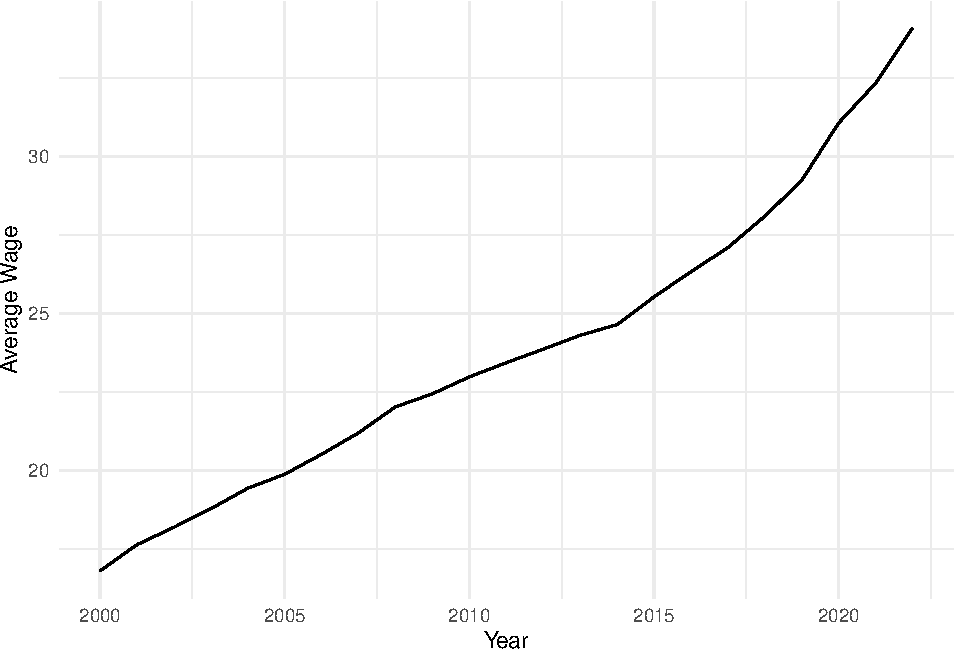
\includegraphics{_main_files/figure-latex/averagewage-1.pdf}
\caption{\label{fig:averagewage}Average Wage}
\end{figure}

The \ref{fig:averagewage} visualization displays the trend of average wages over the two-decade span starting from the year 2000 up to 2023. This plot shows a steady increase in wages, highlighting an upward trajectory that suggests a positive economic trend. The x-axis represents the years, while the y-axis denotes the average wage figures. The line graph is particularly useful for tracking changes over time, making it easier to visualize the rate of growth or any periods of stagnation.

\subsection{Union Wages Comparison by Year}\label{union-wages-comparison-by-year}

Next, we used a boxplot to compare union wages over different years. This gives us a look at how wages have varied for union workers.

\begin{Shaded}
\begin{Highlighting}[]
\FunctionTok{ggplot}\NormalTok{(filtered\_wages, }\FunctionTok{aes}\NormalTok{(}\AttributeTok{x =} \FunctionTok{factor}\NormalTok{(year), }\AttributeTok{y =}\NormalTok{ union\_wage)) }\SpecialCharTok{+}
  \FunctionTok{geom\_boxplot}\NormalTok{() }\SpecialCharTok{+}
  \FunctionTok{labs}\NormalTok{(}\AttributeTok{x =} \StringTok{"Year"}\NormalTok{, }\AttributeTok{y =} \StringTok{"Union Wage"}\NormalTok{) }\SpecialCharTok{+}
  \FunctionTok{theme\_minimal}\NormalTok{()}
\end{Highlighting}
\end{Shaded}

\begin{figure}
\centering
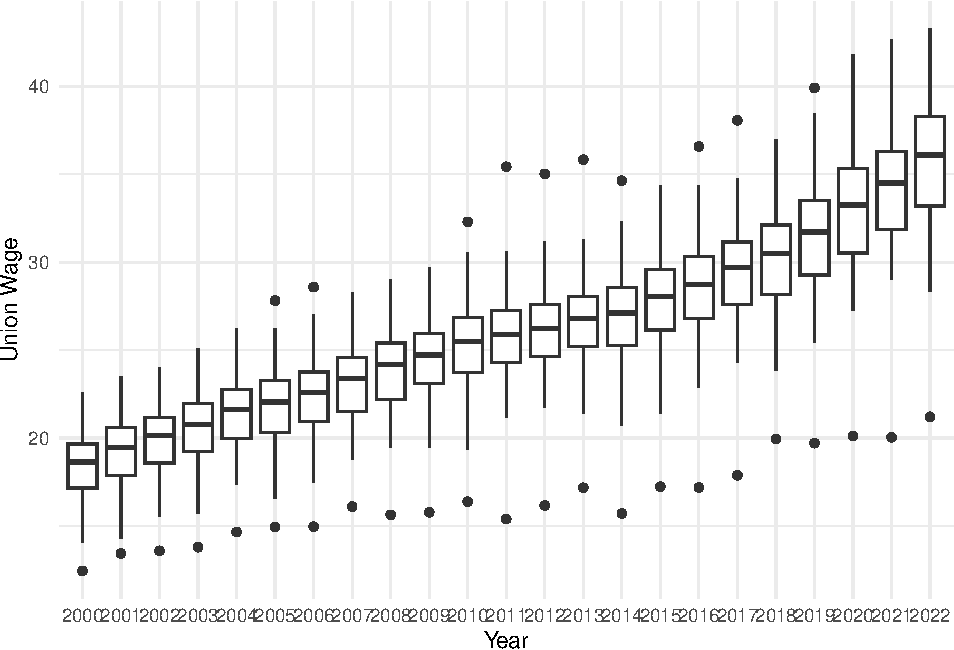
\includegraphics{_main_files/figure-latex/wageyear-1.pdf}
\caption{\label{fig:wageyear}Union Wages by Year}
\end{figure}

This boxplot \ref{fig:wageyear} illustrates union wages over different years, capturing the range of wages as well as median values. By comparing the median line in each box, we can see if union wages have experienced upward or downward trends. The presence of outliers in some years indicates that there were wage values that significantly deviated from the rest of the dataset, providing insights into wage inequality within union jobs. Additionally, the increasing height of the boxes over time may suggest growing wage variability among union workers.

\subsection{Employment Trends by State, Including Union Membership}\label{employment-trends-by-state-including-union-membership}

I wanted to show how employment and union membership vary across different states. For this, we used a combination of bar charts and line graphs. The idea here is to illustrate not just the number of employed people in each state, but also how many of them are union members. This is important because higher union membership often means better wages and working conditions for more people.

\begin{Shaded}
\begin{Highlighting}[]
\FunctionTok{ggplot}\NormalTok{() }\SpecialCharTok{+}
  \FunctionTok{geom\_bar}\NormalTok{(}\AttributeTok{data =}\NormalTok{ states, }\FunctionTok{aes}\NormalTok{(}\AttributeTok{x =}\NormalTok{ state, }\AttributeTok{y =}\NormalTok{ employment), }
           \AttributeTok{stat =} \StringTok{"identity"}\NormalTok{, }\AttributeTok{fill =} \StringTok{"steelblue"}\NormalTok{, }\AttributeTok{alpha =} \FloatTok{0.7}\NormalTok{) }\SpecialCharTok{+}
  \FunctionTok{geom\_line}\NormalTok{(}\AttributeTok{data =}\NormalTok{ merged\_data, }
            \FunctionTok{aes}\NormalTok{(}\AttributeTok{x =}\NormalTok{ state, }\AttributeTok{y =}\NormalTok{ members\_scaled, }
                \AttributeTok{group =}\NormalTok{ state), }\AttributeTok{color =} \StringTok{"red"}\NormalTok{) }\SpecialCharTok{+}
  \FunctionTok{labs}\NormalTok{(}\AttributeTok{x =} \StringTok{"State"}\NormalTok{, }
       \AttributeTok{y =} \StringTok{"Employment/union members"}\NormalTok{, }\AttributeTok{y.sec =} \StringTok{"Members (scaled)"}\NormalTok{) }\SpecialCharTok{+}
  \FunctionTok{theme\_minimal}\NormalTok{() }\SpecialCharTok{+}
  \FunctionTok{scale\_fill\_brewer}\NormalTok{(}\AttributeTok{palette =} \StringTok{"Pastel1"}\NormalTok{) }\SpecialCharTok{+}
  \FunctionTok{coord\_flip}\NormalTok{() }\SpecialCharTok{+}
  \FunctionTok{scale\_y\_continuous}\NormalTok{(}\AttributeTok{sec.axis =} \FunctionTok{sec\_axis}\NormalTok{(}\SpecialCharTok{\textasciitilde{}}\NormalTok{ . }\SpecialCharTok{/} \DecValTok{100}\NormalTok{, }\AttributeTok{name =} \StringTok{"Members"}\NormalTok{))}
\end{Highlighting}
\end{Shaded}

\begin{figure}
\centering
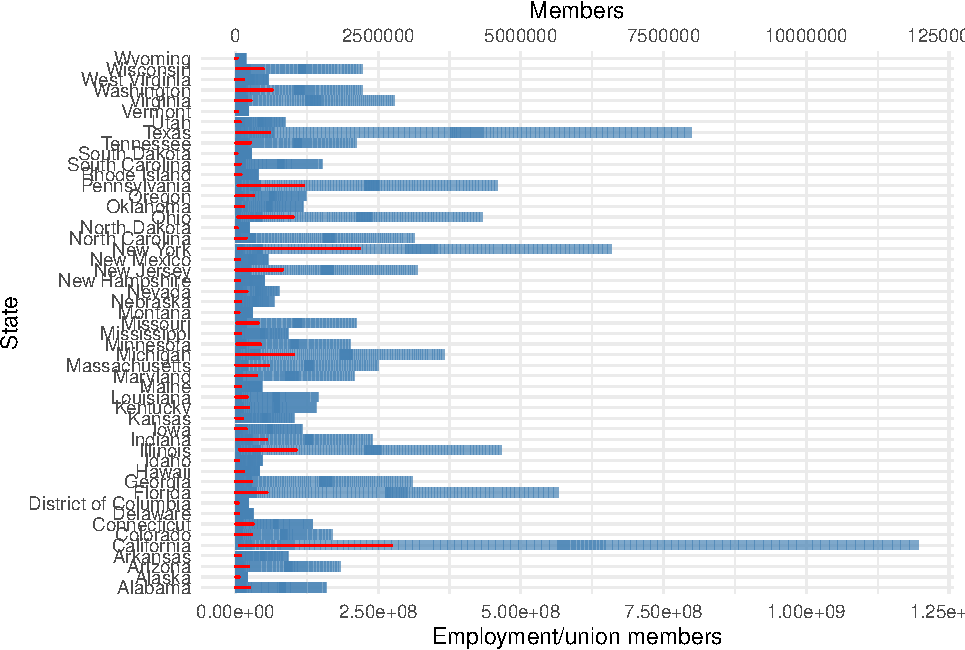
\includegraphics{_main_files/figure-latex/employmenttrend-1.pdf}
\caption{\label{fig:employmenttrend}Employement Trends by State}
\end{figure}

In this graph \ref{fig:employmenttrend}, the blue bars show how many people are working in each state, while the red line shows how many of them are in unions. The states with the highest union membership---like California, New York, and Pennsylvania---are leading the way in worker rights and fair treatment. It's pretty simple: more unions = better lives for workers.

\subsection{Union vs Nonunion Wage Trends Over Time}\label{union-vs-nonunion-wage-trends-over-time}

We wanted to make it crystal clear how much better union wages are compared to nonunion wages. This graph shows just that---union vs.~nonunion wages over time.

\begin{Shaded}
\begin{Highlighting}[]
\FunctionTok{ggplot}\NormalTok{(wages, }\FunctionTok{aes}\NormalTok{(}\AttributeTok{x =}\NormalTok{ year)) }\SpecialCharTok{+}
  \FunctionTok{geom\_smooth}\NormalTok{(}\FunctionTok{aes}\NormalTok{(}\AttributeTok{y =}\NormalTok{ union\_wage, }\AttributeTok{color =} \StringTok{"Union Wage"}\NormalTok{), }
              \AttributeTok{se =} \ConstantTok{FALSE}\NormalTok{, }\AttributeTok{method =} \StringTok{"loess"}\NormalTok{) }\SpecialCharTok{+}
  \FunctionTok{geom\_smooth}\NormalTok{(}\FunctionTok{aes}\NormalTok{(}\AttributeTok{y =}\NormalTok{ nonunion\_wage, }\AttributeTok{color =} \StringTok{"Nonunion Wage"}\NormalTok{), }
              \AttributeTok{se =} \ConstantTok{FALSE}\NormalTok{, }\AttributeTok{method =} \StringTok{"loess"}\NormalTok{) }\SpecialCharTok{+}
  \FunctionTok{labs}\NormalTok{(}\AttributeTok{x =} \StringTok{"Year"}\NormalTok{, }\AttributeTok{y =} \StringTok{"Wage"}\NormalTok{,}
       \AttributeTok{color =} \StringTok{"Type of Wage"}\NormalTok{) }\SpecialCharTok{+}
  \FunctionTok{theme\_minimal}\NormalTok{(}\AttributeTok{base\_size =} \DecValTok{14}\NormalTok{) }\SpecialCharTok{+}
  \FunctionTok{theme}\NormalTok{(}\AttributeTok{legend.position =} \StringTok{"bottom"}\NormalTok{) }\SpecialCharTok{+}
  \FunctionTok{scale\_color\_manual}\NormalTok{(}\AttributeTok{values =} \FunctionTok{c}\NormalTok{(}\StringTok{"Union Wage"} \OtherTok{=} \StringTok{"blue"}\NormalTok{, }\StringTok{"Nonunion Wage"} \OtherTok{=} \StringTok{"green"}\NormalTok{)) }\SpecialCharTok{+}
  \FunctionTok{guides}\NormalTok{(}\AttributeTok{color =} \FunctionTok{guide\_legend}\NormalTok{(}\AttributeTok{title =} \StringTok{"Wage Type"}\NormalTok{))}
\end{Highlighting}
\end{Shaded}

\begin{verbatim}
## `geom_smooth()` using formula = 'y ~ x'
## `geom_smooth()` using formula = 'y ~ x'
\end{verbatim}

\begin{figure}
\centering
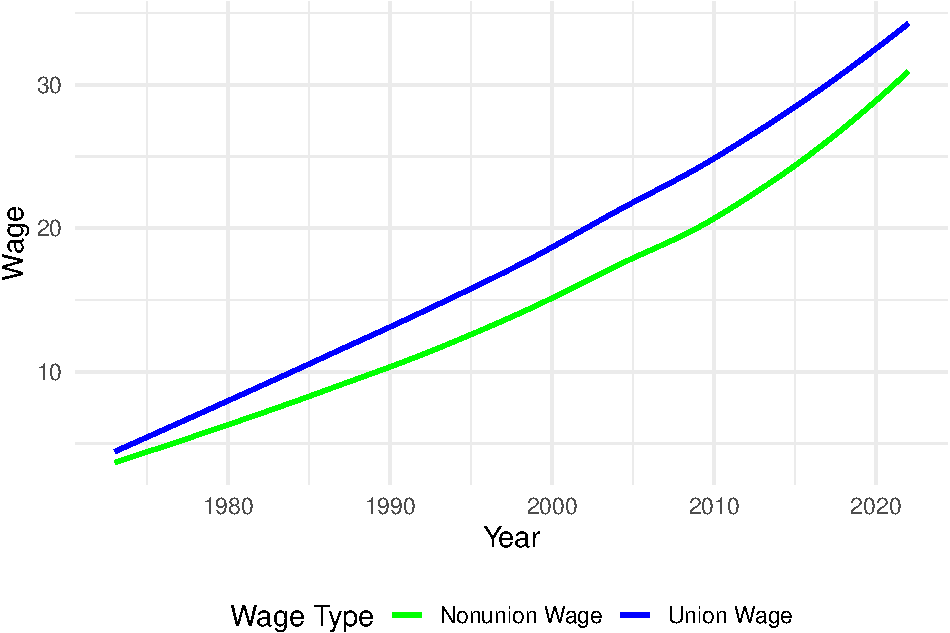
\includegraphics{_main_files/figure-latex/unionvnot-1.pdf}
\caption{\label{fig:unionvnot}Union Vs. Union Wage Over Time}
\end{figure}

Union wages (in blue) are consistently higher than nonunion wages (in green). It's proof that collective bargaining works. When workers join together, they get better pay---it's as simple as that.

\subsection{Union Wage Premium Over Time}\label{union-wage-premium-over-time}

I also took a look at the ``union wage premium,'' which is just a fancy way of saying how much extra money union workers make compared to nonunion workers. This graph shows that premium over time.

\begin{Shaded}
\begin{Highlighting}[]
\FunctionTok{ggplot}\NormalTok{() }\SpecialCharTok{+}
  \FunctionTok{geom\_point}\NormalTok{(}\AttributeTok{data =}\NormalTok{ wages, }\FunctionTok{aes}\NormalTok{(}\AttributeTok{x =}\NormalTok{ year, }\AttributeTok{y =}\NormalTok{ union\_wage\_premium\_raw), }
             \AttributeTok{color =} \StringTok{"orange"}\NormalTok{) }\SpecialCharTok{+}
  \FunctionTok{geom\_smooth}\NormalTok{(}\AttributeTok{data =}\NormalTok{ wages, }
  \FunctionTok{aes}\NormalTok{(}\AttributeTok{x =}\NormalTok{ year, }
      \AttributeTok{y =}\NormalTok{ union\_wage\_premium\_adjusted), }\AttributeTok{method =} \StringTok{"loess"}\NormalTok{, }\AttributeTok{color =} \StringTok{"purple"}\NormalTok{) }\SpecialCharTok{+}
  \FunctionTok{labs}\NormalTok{(}\AttributeTok{x =} \StringTok{"Year"}\NormalTok{, }\AttributeTok{y =} \StringTok{"Wage Premium"}\NormalTok{) }\SpecialCharTok{+}
  \FunctionTok{theme\_minimal}\NormalTok{() }\SpecialCharTok{+}
  \FunctionTok{scale\_color\_brewer}\NormalTok{(}\AttributeTok{palette =} \StringTok{"Dark2"}\NormalTok{)}
\end{Highlighting}
\end{Shaded}

\begin{verbatim}
## `geom_smooth()` using formula = 'y ~ x'
\end{verbatim}

\begin{figure}
\centering
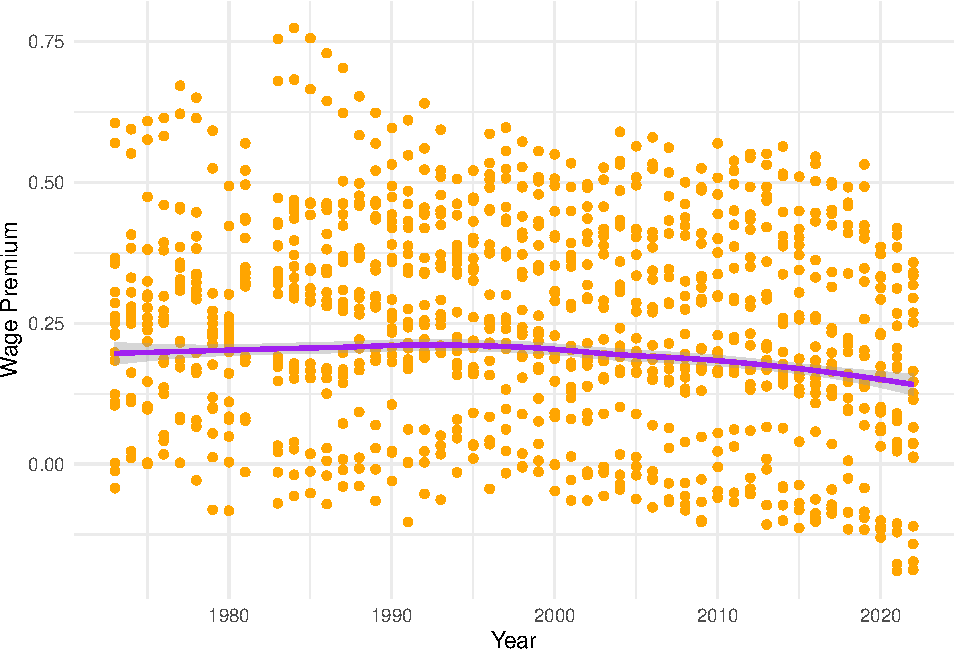
\includegraphics{_main_files/figure-latex/unionpremiumtime-1.pdf}
\caption{\label{fig:unionpremiumtime}Union Wage Premium Over Time}
\end{figure}

The orange points show the raw premium, while the purple line is the adjusted premium. What this graph tells us is that unions are getting workers paid more, even when you take other factors into account. That's real value for workers. But we see that over time this is trending down.

\subsection{Union Membership Trends Over Time}\label{union-membership-trends-over-time}

We also looked at how union membership has changed over time with this area chart. It's important because union membership has been on the decline, and we need to change that.

\begin{Shaded}
\begin{Highlighting}[]
\FunctionTok{ggplot}\NormalTok{(demographics, }\FunctionTok{aes}\NormalTok{(}\AttributeTok{x =}\NormalTok{ year, }\AttributeTok{y =}\NormalTok{ p\_members)) }\SpecialCharTok{+}
  \FunctionTok{geom\_area}\NormalTok{(}\AttributeTok{fill =} \StringTok{"lightblue"}\NormalTok{, }\AttributeTok{alpha =} \FloatTok{0.5}\NormalTok{) }\SpecialCharTok{+}
  \FunctionTok{labs}\NormalTok{(}\AttributeTok{x =} \StringTok{"Year"}\NormalTok{, }\AttributeTok{y =} \StringTok{"Percentage of Union Members"}\NormalTok{) }\SpecialCharTok{+}
  \FunctionTok{theme\_minimal}\NormalTok{() }\SpecialCharTok{+}
  \FunctionTok{scale\_fill\_brewer}\NormalTok{(}\AttributeTok{palette =} \StringTok{"Blues"}\NormalTok{)}
\end{Highlighting}
\end{Shaded}

\begin{figure}
\centering
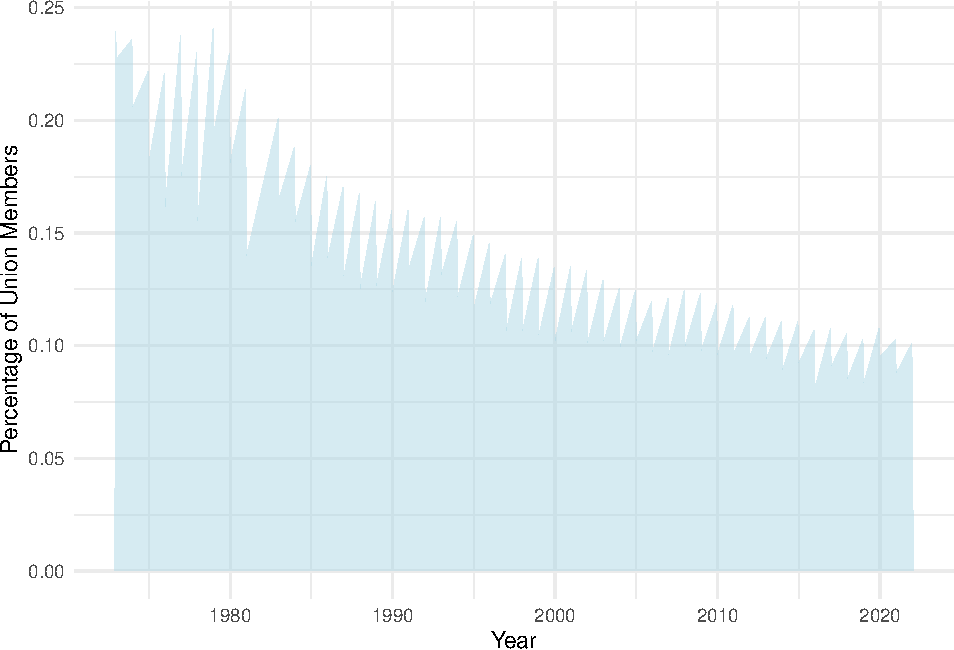
\includegraphics{_main_files/figure-latex/membertime-1.pdf}
\caption{\label{fig:membertime}Uniont Membership Trends}
\end{figure}

The drop in union membership is clear. Fewer union members mean less bargaining power, and that's why wages haven't risen as fast as they should. We need to support union growth to bring back fair wages and worker protections.

\subsection{Employment in Different Sectors Over Time}\label{employment-in-different-sectors-over-time}

Lastly, we looked at employment trends across different sectors. This stacked bar graph shows how employment has changed from manufacturing to more service-focused jobs over time.

\begin{Shaded}
\begin{Highlighting}[]
\FunctionTok{ggplot}\NormalTok{(states, }\FunctionTok{aes}\NormalTok{(}\AttributeTok{x =}\NormalTok{ year, }\AttributeTok{y =}\NormalTok{ employment, }\AttributeTok{fill =}\NormalTok{ sector)) }\SpecialCharTok{+}
  \FunctionTok{geom\_bar}\NormalTok{(}\AttributeTok{stat =} \StringTok{"identity"}\NormalTok{, }\AttributeTok{position =} \StringTok{"stack"}\NormalTok{) }\SpecialCharTok{+}
  \FunctionTok{labs}\NormalTok{(}\AttributeTok{x =} \StringTok{"Year"}\NormalTok{, }\AttributeTok{y =} \StringTok{"Employment"}\NormalTok{) }\SpecialCharTok{+}
  \FunctionTok{theme\_minimal}\NormalTok{() }\SpecialCharTok{+}
  \FunctionTok{scale\_fill\_brewer}\NormalTok{(}\AttributeTok{palette =} \StringTok{"Spectral"}\NormalTok{)}
\end{Highlighting}
\end{Shaded}

\begin{figure}
\centering
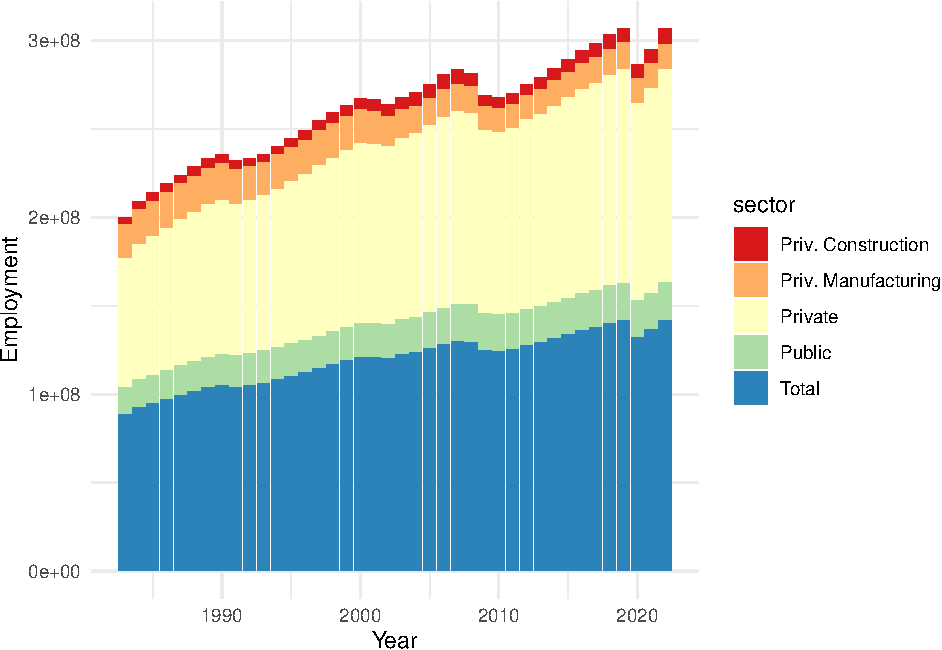
\includegraphics{_main_files/figure-latex/sectoremploy-1.pdf}
\caption{\label{fig:sectoremploy}Setor Employement}
\end{figure}

The private sector---especially services---has grown a lot, while manufacturing has shrunk. We need unions in all these sectors to keep fighting for fair pay and worker rights, no matter what kind of work people are doing.

\section{Discussion and Summary}\label{discussion-and-summary}

\subsection{Wage Growth and Union Influence}\label{wage-growth-and-union-influence}

Une thing is crystal clear: union workers make more money. The graphs and numbers show that if you're in a union, you're getting paid better compared to folks who aren't. We're talking about both the raw numbers (the difference in pay) and the adjusted numbers (where we consider factors like age, job type, etc.). And guess what? Even when you adjust for those things, union workers still come out on top.

When we looked at the trends over time, union wages have consistently been higher. Sure, there's been some narrowing of the gap lately, but unions are still the best bet for fair wages. If unions start losing power, everyone's pay could start sliding back. We need to keep unions strong if we want to keep fighting for better wages for all workers.

\subsection{Decline in Union Membership}\label{decline-in-union-membership}

One of the more worrying things we saw is how union membership has been dropping for the past couple of decades. There are a bunch of reasons for this. The economy has shifted---manufacturing, where unions were strong, has shrunk, and we've moved towards more service jobs, which are harder to organize. Plus, with globalization, a lot of jobs went overseas or became automated, and that took away a lot of union power.

And let's not forget the gig economy. More and more people are working gig jobs or part-time, which makes it tough for them to organize and join unions. Fewer unions mean less power for workers to negotiate fair pay and benefits, and that's not good for anyone. If we want to turn this around, we need to make it easier for workers in all kinds of jobs to join unions and fight for their rights.

\subsection{Shifts in Employment by Sector}\label{shifts-in-employment-by-sector}

Another big trend we saw is that employment has shifted from industries like manufacturing and construction into the service sector. The service industry has been booming, but it hasn't been easy for unions to gain a foothold there. That means a lot of workers in service jobs are missing out on the protections and pay boosts that unions can provide.

The public sector is one of the few places where unions are still doing okay, but even there, unions are under pressure from budget cuts and changes to policies that aim to cut spending. If we want to improve job quality for everyone, unions need to find ways to grow in these new industries. The service sector needs unions more than ever to help protect workers' rights and improve their pay.

\subsection{Implications for the Future}\label{implications-for-the-future}

So, what does all this mean for the future? Well, we've got some challenges, but also opportunities. Unions are still crucial for securing better wages, but the decline in membership is a problem we need to solve. The answer might be new organizing strategies---unions need to adapt to reach workers in tech, service, and gig industries. If unions can innovate, they can still be a powerful force for worker rights.

If union membership keeps shrinking, we're going to see more income inequality. That means the gap between the rich and the poor will get wider, and that's bad news for everyone. Unions help level the playing field, so we need to support them, whether through better labor laws or by organizing in new industries.

The shift to more service-based jobs could be an opportunity if unions can step in and start organizing those workers. The future of the labor market is going to depend a lot on how well unions, workers, and policymakers can adapt to these changes. We need to work together to make sure everyone gets fair wages and decent working conditions, no matter where they work.

Unions have always been about making things fair for workers, and that mission hasn't changed. We need to keep building union power to make sure everyone gets a fair shake in this rapidly changing economy.

  \bibliography{book.bib}

\end{document}
